\section{Euclidean Spaces and Lattices}
\begin{enumerate}
	\item
	\begin{proof}[\normalfont\color{magenta}\bfseries Sol]
%		\begin{align*}
%			\langle \mathbf{x},\mathbf{y}\rangle
%			&=
%			(1)(4)+(-2)(0)+(3)(-1)=4+0-3=1.\\
%			\|\mathbf{x}\|
%			&=
%			\sqrt{1^2+(-2)^2+3^2}
%			=\sqrt{1+4+9}
%			=\sqrt{14}.\\
%			\|\mathbf{y}\|
%			&=\sqrt{4^2+0^2+(-1)^2}
%			=\sqrt{16+0+1}
%			=\sqrt{17}.\\
%			\mathbf{x}+\mathbf{y}&=(1+4,-2+0,3+(-1))=(5,-2,2),\\
%			\|\mathbf{x}+\mathbf{y}\|
%			&=\sqrt{5^2+(-2)^2+2^2}
%			=\sqrt{25+4+4}
%			=\sqrt{33}.
%		\end{align*}
%		Therefore,
		\[
		\boxed{
			\langle \mathbf{x},\mathbf{y}\rangle=1,\qquad
			\|\mathbf{x}\|=\sqrt{14},\qquad
			\|\mathbf{y}\|=\sqrt{17},\qquad
			\|\mathbf{x}+\mathbf{y}\|=\sqrt{33}.
		}
		\]
	\end{proof}
	\item[]
	\item
	\begin{proof}[\normalfont\color{magenta}\bfseries Sol]
		\begin{enumerate}
			\item Yes, this is a lattice. Indeed,
			\[
			\mathbb{Z}^2
			=
			\{a(1,0)+b(0,1):a,b\in\mathbb{Z}\}=\mathcal L(\textbf{e}_1,\textbf{e}_2).
			\]
			
			\item Yes, this is a lattice of rank \(1\) in \(\mathbb{R}^2\). We may write it as
			\[
			\{a(1,\sqrt{2}):a\in\mathbb{Z}\}=\mathcal L(1,\sqrt{2}).
			\]
			%		It is the set of integer multiples of the nonzero vector \((1,\sqrt{2})\), so it is a discrete subgroup lying on a line.
			
			\item Yes, this is a lattice in \(\mathbb{R}^2\).
			\[
			\{a(1,0)+b(1/2,1): a,b\in\mathbb{Z}\}=\mathcal L(\textbf{b}_1,\textbf{b}_2)\quad\text{where}\quad\mathbf{b}_1=(1,0),\qquad \mathbf{b}_2=\left(\frac12,1\right).
			\]
			
			\item No, this is not a lattice. 
			%		Although \(\mathbb{Q}^2\) is closed under addition and negation, it is not discrete in \(\mathbb{R}^2\). Indeed, 
			There are rational points arbitrarily close to \((0,0)\), for example
			\[
			\left(\frac1n,0\right)\in\mathbb{Q}^2
			\qquad\text{for all }n\in\mathbb{N},
			\]
			and these converge to \((0,0)\). Hence \(\mathbb{Q}^2\) is not a lattice.
		\end{enumerate}
		
		Therefore:
		\[
		\boxed{
			\mathbb{Z}^2,\ \{(a,\sqrt2 a):a\in\mathbb Z\},\ \{a(1,0)+b(1/2,1):a,b\in\mathbb Z\}
			\text{ are lattices, but }\mathbb Q^2\text{ is not.}
		}
		\]
	\end{proof}
	\newpage
	\item \begin{proof}[\normalfont\color{magenta}\bfseries Sol]
		The real span is
		\[
		\operatorname{span}_{\mathbb R}\{\mathbf{b}_1,\mathbf{b}_2\}
		=
		\left\{
		a\begin{pmatrix}2\\0\end{pmatrix}
		+
		b\begin{pmatrix}1\\1\end{pmatrix}
		:a,b\in\mathbb R
		\right\}.
		\]
		Computing,
		\[
		a\begin{pmatrix}2\\0\end{pmatrix}
		+
		b\begin{pmatrix}1\\1\end{pmatrix}
		=
		\begin{pmatrix}
			2a+b\\
			b
		\end{pmatrix}.
		\]
		Given any \((x,y)\in\mathbb R^2\), choose \(b=y\) and \(a=(x-y)/2\). Hence every vector in \(\mathbb R^2\) has this form, so
		\[
		\operatorname{span}_{\mathbb R}\{\mathbf{b}_1,\mathbf{b}_2\}=\mathbb R^2.
		\]
		
		The lattice generated by \(\mathbf{b}_1,\mathbf{b}_2\) is
		\[
		\Lambda
		=
		\left\{
		m\begin{pmatrix}2\\0\end{pmatrix}
		+
		n\begin{pmatrix}1\\1\end{pmatrix}
		:m,n\in\mathbb Z
		\right\}
		=
		\left\{
		\begin{pmatrix}
			2m+n\\
			n
		\end{pmatrix}
		:m,n\in\mathbb Z
		\right\}.
		\]
		Equivalently,
		\[
		\Lambda=\{(x,y)\in\mathbb Z^2:x-y\in 2\mathbb Z\}
		=\{(x,y)\in\mathbb Z^2:x\equiv y\pmod{2}\}.
		\]
		So the lattice consists of all integer points whose coordinates have the same parity.
		Therefore,
		\[
		\boxed{
			\operatorname{span}_{\mathbb R}\{\mathbf b_1,\mathbf b_2\}=\mathbb R^2,
			\qquad
			\Lambda=
			\left\{
			\begin{pmatrix}
				2m+n\\
				n
			\end{pmatrix}
			:m,n\in\mathbb Z
			\right\}.
		}
		\]
	\end{proof}
	
	
	
	\begin{center}
		\begin{tikzpicture}[scale=1.1, >=Stealth]
			
			% Axes
			\draw[->, thick] (-3.5,0) -- (5.5,0) node[right] {$x$};
			\draw[->, thick] (0,-3.5) -- (0,4.5) node[above] {$y$};
			
			% Grid
			\draw[step=1cm, gray!25, very thin] (-3.5,-3.5) grid (5.5,4.5);
			
			% Span of b1
			\draw[blue, thick] (-3.3,0) -- (5.3,0)
			node[pos=0.9, below] {$\operatorname{span}_{\mathbb R}(b_1)$};
			
			% Span of b2
			\draw[red, thick] (-3.2,-3.2) -- (4.2,4.2)
			node[pos=0.82, above left] {$\operatorname{span}_{\mathbb R}(b_2)$};
			
			% Vectors
			\draw[->, very thick, blue!80!black] (0,0) -- (2,0)
			node[midway, below] {$b_1$};
			
			\draw[->, very thick, red!80!black] (0,0) -- (1,1)
			node[midway, left] {$b_2$};
			
			% Lattice points
			\foreach \x in {-3,-2,-1,0,1,2,3,4,5} {
				\foreach \y in {-3,-2,-1,0,1,2,3,4} {
					\pgfmathtruncatemacro{\parity}{mod(\x-\y,2)}
					\ifnum\parity=0
					\fill[black] (\x,\y) circle (2.2pt);
					\fi
				}
			}
			
		\end{tikzpicture}
	\end{center}
	\item 
	\begin{proof}[\normalfont\color{magenta}\bfseries Sol]
		We first show that \(\Lambda\) is a subgroup of \((\mathbb{R}^n,+)\).
		If
		\[
		\mathbf{x}=\sum_{i=1}^m z_i\mathbf{b}_i,
		\qquad
		\mathbf{y}=\sum_{i=1}^m w_i\mathbf{b}_i
		\]
		are in \(\Lambda\), with \(z_i,w_i\in\mathbb Z\), then
		\[
		\mathbf{x}-\mathbf{y}
		=
		\sum_{i=1}^m (z_i-w_i)\mathbf{b}_i.
		\]
		Since \(z_i-w_i\in\mathbb Z\), we have \(\mathbf{x}-\mathbf{y}\in\Lambda\).
		
		\medskip
		\noindent
		Let
		\[
		V=\operatorname{span}_{\mathbb R}\{\mathbf{b}_1,\dots,\mathbf{b}_m\}.
		\]
		Since the vectors are linearly independent, the map
		\[
		T:\mathbb R^m\to V,\qquad
		T(z_1,\dots,z_m)=\sum_{i=1}^m z_i\mathbf{b}_i
		\]
		is a linear isomorphism. In particular, \(T(\mathbb Z^m)=\Lambda\).
		Because \(\mathbb Z^m\) is discrete in \(\mathbb R^m\), and \(T\) is a homeomorphism from \(\mathbb R^m\) onto \(V\), it follows that \(\Lambda\) is discrete in \(V\), hence also discrete in \(\mathbb R^n\).
		Therefore \(\Lambda\) is a discrete subgroup of \(\mathbb R^n\).
	\end{proof}
	\item[]
	\item 
	\begin{proof}[\normalfont\color{magenta}\bfseries Sol]
		Consider the standard lattice
		\[
		\mathbb Z^2.
		\]
		One basis is
		\[
		\mathbf b_1=(1,0),\qquad \mathbf b_2=(0,1).
		\]
		Another basis is
		\[
		\mathbf c_1=(1,1),\qquad \mathbf c_2=(1,0).
		\]
		Indeed,
		\[
		\mathbf c_1=(1,1),\qquad \mathbf c_2=(1,0)
		\]
		are linearly independent, and every integer vector \((x,y)\in\mathbb Z^2\) can be written as
		\[
		(x,y)=y(1,1)+(x-y)(1,0).
		\]
		Since \(x,y\in\mathbb Z\), this is an integer linear combination of \(\mathbf c_1,\mathbf c_2\). Hence
		\[
		\mathbb Z^2=\mathcal L(\mathbf b_1,\mathbf b_2)=\mathcal L(\mathbf c_1,\mathbf c_2).
		\]
		
		Thus two distinct bases of the same lattice are
		\[
		\boxed{
			\{(1,0),(0,1)\}
			\qquad\text{and}\qquad
			\{(1,1),(1,0)\}.
		}
		\]
	\end{proof}
	
	\newpage
	\item 
	\begin{proof}[\normalfont\color{magenta}\bfseries Sol]
		The lattice generated by \(\mathbf{b}_1,\mathbf{b}_2\) is
		\[
		\mathcal L(B)
		=
		\{z_1\mathbf{b}_1+z_2\mathbf{b}_2 : z_1,z_2\in\mathbb{Z}\}.
		\]
		
		Substituting the basis vectors,
		\[
		\mathcal L(B)
		=
		\left\{
		z_1
		\begin{pmatrix}
			1\\2
		\end{pmatrix}
		+
		z_2
		\begin{pmatrix}
			3\\4
		\end{pmatrix}
		: z_1,z_2\in\mathbb{Z}
		\right\}.
		\]
		
		Thus
		\[
		\mathcal L(B)
		=
		\left\{
		\begin{pmatrix}
			z_1+3z_2\\
			2z_1+4z_2
		\end{pmatrix}
		: z_1,z_2\in\mathbb{Z}
		\right\}.
		\]
		
		So explicitly,
		\[
		\boxed{
			\mathcal L(B)
			=
			\left\{
			(x,y)\in\mathbb{R}^2 :
			x=z_1+3z_2,\;
			y=2z_1+4z_2,\;
			z_1,z_2\in\mathbb{Z}
			\right\}.
		}
		\]
		
		%	\bigskip
		
		\begin{center}
			\begin{tikzpicture}[scale=0.7, >=Stealth]
				
				% Axes
				\draw[->, thick] (-8.5,0) -- (8.5,0) node[right] {$x$};
				\draw[->, thick] (0,-8.5) -- (0,8.5) node[above] {$y$};
				
				% Grid
				\draw[step=1cm, gray!25, very thin] (-8.5,-8.5) grid (8.5,8.5);
				
				% Lattice points: m*b1 + n*b2 = (m+3n, 2m+4n)
				\foreach \m in {-3,-2,-1,0,1,2,3} {
					\foreach \n in {-3,-2,-1,0,1,2,3} {
						\pgfmathsetmacro{\X}{\m + 3*\n}
						\pgfmathsetmacro{\Y}{2*\m + 4*\n}
						\ifdim \X pt > -8.2pt
						\ifdim \X pt < 8.2pt
						\ifdim \Y pt > -8.2pt
						\ifdim \Y pt < 8.2pt
						\fill[black] (\X,\Y) circle (2.2pt);
						\fi
						\fi
						\fi
						\fi
					}
				}
				
				% Basis vectors
				\draw[->, very thick, blue!80!black] (0,0) -- (1,2)
				node[midway, left] {$\mathbf{b}_1$};
				
				\draw[->, very thick, red!80!black] (0,0) -- (3,4)
				node[midway, right] {$\mathbf{b}_2$};
				
				% Fundamental parallelogram
				\draw[dashed, thick, purple] (0,0) -- (1,2) -- (4,6) -- (3,4) -- cycle;
				
				% Labels
				\node[fill=white, inner sep=2pt] at (5.2,6.7) {$\mathbf{b}_1+\mathbf{b}_2$};
				\node[fill=white, inner sep=2pt] at (5.8,-6.8)
				{$\mathcal L(B)=\left\{\binom{z_1+3z_2}{2z_1+4z_2}:z_1,z_2\in\mathbb{Z}\right\}$};
				
			\end{tikzpicture}
		\end{center}
	\end{proof}
	\newpage
	\item 
	\begin{proof}[\normalfont\color{magenta}\bfseries Sol]
		Consider the lattice \(\mathbb Z^2\). For each integer \(k\in\mathbb Z\), define
		\[
		\mathbf b_1^{(k)}=(1,0),
		\qquad
		\mathbf b_2^{(k)}=(k,1).
		\]
		Then
		\[
		B_k=
		\begin{pmatrix}
			1 & k\\
			0 & 1
		\end{pmatrix}
		\]
		has \(\det (B_k)=1\), so its columns form a basis of \(\mathbb Z^2\).	
		Indeed, every vector in \(\mathcal L(B_k)\) has the form
		\[
		a(1,0)+b(k,1)=(a+bk,b),
		\qquad a,b\in\mathbb Z.
		\]
		Given any \((x,y)\in\mathbb Z^2\), choose \(b=y\) and \(a=x-ky\). Then
		\[
		(x,y)=a(1,0)+b(k,1),
		\]
		so \(\mathcal L(B_k)=\mathbb Z^2\).	As \(k\) varies over \(\mathbb Z\), these bases are distinct. Therefore the lattice \(\mathbb Z^2\) has infinitely many bases.
		Hence a lattice may have infinitely many bases.
	\end{proof}
	\item 
	\begin{proof}[\normalfont\color{magenta}\bfseries Sol]
		Suppose
		\[
		\Lambda=\left\{\sum_{i=1}^m z_i\mathbf b_i:z_i\in\mathbb Z\right\}
		\]
		for some linearly independent vectors \(\mathbf b_1,\dots,\mathbf b_m\in\mathbb R^n\).
		Define the map
		\[
		f:\mathbb Z^m\to\Lambda,
		\qquad
		f(z_1,\dots,z_m)=\sum_{i=1}^m z_i\mathbf b_i.
		\]
		This map is surjective by definition of \(\Lambda\). Since \(\mathbb Z^m\) is countable, and the image of a countable set under a map is countable, it follows that \(\Lambda\) is countable.
		Therefore every lattice is countable.
	\end{proof}
	\item 
	\begin{proof}[\normalfont\color{magenta}\bfseries Sol]
		Let
		\[
		\Lambda=\left\{\sum_{i=1}^m z_i\mathbf b_i:z_i\in\mathbb Z\right\}.
		\]
		First, \(\Lambda\) contains the zero vector because taking all coefficients equal to \(0\) gives
		\[
		\mathbf 0=\sum_{i=1}^m 0\cdot \mathbf b_i\in\Lambda.
		\]
		Now let
		\[
		\mathbf x=\sum_{i=1}^m z_i\mathbf b_i,
		\qquad
		\mathbf y=\sum_{i=1}^m w_i\mathbf b_i
		\]
		be vectors in \(\Lambda\). Then
		\[
		\mathbf x+\mathbf y
		=
		\sum_{i=1}^m (z_i+w_i)\mathbf b_i.
		\]
		Since \(z_i+w_i\in\mathbb Z\), we have \(\mathbf x+\mathbf y\in\Lambda\). Thus \(\Lambda\) is closed under addition.
		Also,
		\[
		-\mathbf x
		=
		\sum_{i=1}^m (-z_i)\mathbf b_i.
		\]
		Since \(-z_i\in\mathbb Z\), it follows that \(-\mathbf x\in\Lambda\). Thus \(\Lambda\) is closed under negation.
		Therefore every lattice contains \(\mathbf 0\) and is closed under addition and negation.
	\end{proof}
	\item 
	\begin{proof}[\normalfont\color{magenta}\bfseries Sol]
		We rewrite the general element of \(\Lambda\) as 
		\[
		\Lambda=\{a(2,0)+b(1,1):a,b\in\mathbb Z\}.
		\]
		So a basis matrix is obtained by taking these vectors as columns:
		\[
		B=
		\begin{pmatrix}
			2 & 1\\
			0 & 1
		\end{pmatrix}.
		\]
		Then
		\[
		B\begin{pmatrix}a\\ b\end{pmatrix}
		=
		\begin{pmatrix}
			2 & 1\\
			0 & 1
		\end{pmatrix}
		\begin{pmatrix}
			a\\ b
		\end{pmatrix}
		=
		\begin{pmatrix}
			2a+b\\
			b
		\end{pmatrix}.
		\]
		Therefore
		\[
		\boxed{
			B=
			\begin{pmatrix}
				2 & 1\\
				0 & 1
			\end{pmatrix}
		}
		\qquad\text{and}\qquad
		\Lambda=\mathcal L(B).
		\]
	\end{proof}
\end{enumerate}

\section{Gram--Schmidt Orthogonalization}

\newpage
\section{Fundamental Parallelepipeds and Determinants}

\begin{enumerate}
\item[\textbf{21-24}] We are given
\[
B=
\begin{pmatrix}
	2&1\\
	0&3
\end{pmatrix},
\qquad
\Lambda=\mathcal L(B),
\qquad
\mathcal P(B)=\{B\boldsymbol\alpha:\boldsymbol\alpha\in[0,1)^2\}.
\]
The columns of \(B\) are
\[
\mathbf b_1=\binom{2}{0},
\qquad
\mathbf b_2=\binom{1}{3},\qquad\text{so}\qquad B=	\begin{pmatrix}
	\textbf{b}_1&\textbf{b}_2
\end{pmatrix}.
\]
\begin{center}
	\begin{tikzpicture}[>=stealth, scale=0.9, transform shape]
		% Define common point styles
		\tikzstyle{pt} = [circle, fill=black, inner sep=1.8pt];
		\tikzstyle{targetpt} = [circle, fill=red, inner sep=1.8pt];
		
		% =========================================================================
		% LEFT SIDE: Standard Space R^2 (Variables: z, t, alpha)
		% =========================================================================
		\begin{scope}[xshift=0cm, yshift=0cm]
			% -- Standard Grid Lines --
			% These lines represent the integer grid of Z^2
			\draw[step=1cm, gray!60, thin] (-0.5,-0.5) grid (4.5,3.5);
			% -- Axes --
			\draw[->, thick] (-0.5,0) -- (4.5,0) node[right] {$x_1$};
			\draw[->, thick] (0,-0.5) -- (0,3.5) node[above] {$x_2$};
			
			% -- Highlighted Regions --
			% 1. Standard Fundamental Domain [0,1)^2 at origin
			\fill[green!15, opacity=0.7] (0,0) rectangle (1,1);
			\draw[green!50!black, thick] (0,1) -- (0,0) -- (1,0); 
			\draw[green!50!black, thick, dashed] (1,0) -- (1,1) -- (0,1);
			\node[text=green!50!black] at (2.25, .5) {\small $\mathcal{P}(I)=[0,1)^2$};
			
			% -- Draw Integer Lattice Points Z^2 --
			\foreach \x in {0,...,4} {
				\foreach \y in {0,...,3} {
						\fill[black] (\x,\y) circle (1.5pt);
					}
			}
			\draw[blue, thick, ->] (0,0) -- (1,0); 
			\draw[blue, thick, ->] (0,0) -- (0,1); 
			\filldraw[blue] (1,0) circle (2pt) node[right] {$\textbf{b}_1$}; 
			\filldraw[blue] (0,1) circle (2pt) node[above] {$\textbf{b}_2$}; 
		\end{scope}
		
		% =========================================================================
		% MAPPING ARROW
		% =========================================================================
		\draw[->, line width=1.5pt] (6, 1.5) -- (8, 1.5) 
		node[midway, above, text=black] {\small $B = \begin{pmatrix} 2 & 1 \\ 0 & 3 \end{pmatrix}$};
		
		% =========================================================================
		% RIGHT SIDE: Transformed Space R^2 (Variables: Bz, x, B alpha)
		% =========================================================================
		\begin{scope}[xshift=9.5cm]
			% -- Background Standard Grid (Faint) --
			\draw[gray!15, very thin, step=1cm] (-0.5,-0.5) grid (6.5, 3.5);
			% -- Axes --
			\draw[->, thick] (-0.5,0) -- (6.5,0) node[right] {$x_1$};
			\draw[->, thick] (0,-0.5) -- (0,3.5) node[above] {$x_2$};
			
			% We use a local scope with basis vectors mapped by B
			\begin{scope}[x={(2cm,0cm)}, y={(1cm,3cm)}]	
				% -- NEW SKEWED GRID LINES --

				% Lines parallel to B*e_2 (the "vertical" skewed lines)
				\foreach \i in {0,1,2,3} {
					\draw[gray!60, thin] (\i, -0.2) -- (\i, 1.2);
				}
				% Lines parallel to B*e_1 (the "horizontal" skewed lines)
				\foreach \j in {1} {
					\draw[gray!60, thin] (-0.5, \j) -- (3, \j);
				}
			
				% -- Draw Transformed Lattice Points Lambda --
				\foreach \i in {0,...,3} {
					\foreach \j in {0,...,1} {
							% Draw points only if they fit within the visual axes bounds
							\pgfmathsetmacro{\xpos}{2*\i + \j}
							\pgfmathsetmacro{\ypos}{3*\j}
							\ifdim \xpos pt < 8.2pt \ifdim \ypos pt < 6.2pt
							\fill[black] (\i,\j) circle (1.5pt);
							\fi\fi
						}
				}
				
				% -- Highlighted Regions --
				% 1. Fundamental Parallelepiped P(B) at origin
				\fill[green!15, opacity=0.7] (0,0) -- (1,0) -- (1,1) -- (0,1) -- cycle;
				\fill[green!15, opacity=0.7] (0,0) -- (1,0) -- (1,1) -- (0,1) -- cycle;
				\draw[green!50!black, thick] (0,1) -- (0,0) -- (1,0); 
				\draw[green!50!black, thick, dashed] (1,0) -- (1,1) -- (0,1);
				\node[text=green!50!black] at (0.5, -0.15) {\small $\mathcal{P}(B)$};
				\draw[red, thick, ->] (0,0) -- (1,0); 
				\draw[red, thick, ->] (0,0) -- (0,1); 
				\filldraw[red] (1,0) circle (2pt) node[right] {$\textbf{b}_1$}; 
				\filldraw[red] (0,1) circle (2pt) node[above] {$\textbf{b}_2$}; 
			\end{scope}
		\end{scope}
	\end{tikzpicture}
\end{center}
\end{enumerate}

\begin{enumerate}
	\setcounter{enumi}{20}
	\item \begin{proof}[\normalfont\color{magenta}\bfseries Sol]
	Since
	\[
	\det(B)=2\cdot 3-0\cdot 1=6,
	\]
	we have
	\[
	B^{-1}
	=
	\frac1{6}
	\begin{pmatrix}
		3&-1\\
		0&2
	\end{pmatrix}
	=
	\begin{pmatrix}
		\frac12&-\frac16\\[4pt]
		0&\frac13
	\end{pmatrix}.
	\]
	
	Thus
	\[
	\boxed{
		B^{-1}
		=
		\begin{pmatrix}
			\frac12&-\frac16\\[4pt]
			0&\frac13
		\end{pmatrix}.
	}
	\]
	\end{proof}
	\item \begin{proof}[\normalfont\color{magenta}\bfseries Sol]
	\begin{enumerate}
		\item Write $
		\mathbf x=\begin{pmatrix}
			7.4 \\ 5.2
		\end{pmatrix}=\begin{pmatrix}\frac{37}{5}\\ \frac{26}{5}\end{pmatrix}$.
		Then
		\[
		\mathbf t
		=
		B^{-1}\mathbf x
		=
		\begin{pmatrix}
			\frac12&-\frac16\\[4pt]
			0&\frac13
		\end{pmatrix}
		\begin{pmatrix}\frac{37}{5}\\ \frac{26}{5}\end{pmatrix}
		=
		\begin{pmatrix}\frac{17}{6}\\ \frac{26}{15}\end{pmatrix}.
		\]
		Hence
		\[
		\mathbf z=\left\lfloor \mathbf t\right\rfloor
		=
		\begin{pmatrix}2 \\ 1\end{pmatrix},
		\qquad
		\boldsymbol\alpha
		=
		\mathbf t-\mathbf z
		=
		\begin{pmatrix}\frac56 \\ \frac{11}{15}\end{pmatrix}.
		\]
		Therefore
		\[
		B\mathbf z
		=
		\begin{pmatrix}
			2&1\\
			0&3
		\end{pmatrix}
		\begin{pmatrix}2 \\ 1\end{pmatrix}=
		\begin{pmatrix}5 \\ 3\end{pmatrix},\qquad\text{and}\qquad
		B\boldsymbol\alpha
		=
		\begin{pmatrix}
			2&1\\
			0&3
		\end{pmatrix}
		\begin{pmatrix}\frac56 \\ \frac{11}{15}\end{pmatrix}
		=
		\begin{pmatrix}\frac{12}{5} \\ \frac{11}{5}\end{pmatrix}.
		\]
		So
		\[
		\boxed{
			\begin{pmatrix}{7.4}\\ {5.2}\end{pmatrix}
			=
			\begin{pmatrix}{5}\\ {3}\end{pmatrix}
			+
			\begin{pmatrix}{\frac{12}{5}}\\ {\frac{11}{5}}\end{pmatrix}.
		}
		\]
		\begin{center}
	\begin{tikzpicture}[>=stealth, scale=0.8, transform shape]
		% Define common point styles
		\tikzstyle{pt} = [circle, fill=black, inner sep=1.8pt];
		\tikzstyle{targetpt} = [circle, fill=red, inner sep=1.8pt];
		
		% =========================================================================
		% LEFT SIDE: Standard Space R^2 (Variables: z, t, alpha)
		% =========================================================================
		\begin{scope}[xshift=0cm, yshift=1.5cm]
			% -- Standard Grid Lines --
			% These lines represent the integer grid of Z^2
			\draw[step=1cm, gray!60, thin] (-0.5,-0.5) grid (4.5,3.5);
			% -- Axes --
			\draw[->, thick] (-0.5,0) -- (4.5,0) node[right] {$x_1$};
			\draw[->, thick] (0,-0.5) -- (0,3.5) node[above] {$x_2$};
		
			% -- Highlighted Regions --
			% 1. Standard Fundamental Domain [0,1)^2 at origin
			\fill[green!15, opacity=0.7] (0,0) rectangle (1,1);
			\draw[green!50!black, thick] (0,1) -- (0,0) -- (1,0); 
			\draw[green!50!black, thick, dashed] (1,0) -- (1,1) -- (0,1);
			\node[text=green!50!black] at (1.25, -.5) {\small $\mathcal{P}(I)=[0,1)^2$};
			
			% 2. Specific Translated Domain z + [0,1)^2 containing vector t
			\fill[blue!15, opacity=0.7] (2,1) rectangle (3,2);
			\draw[blue, thick] (2,2) -- (2,1) -- (3,1); 
			\draw[blue, thick, dashed] (3,1) -- (3,2) -- (2,2);
			\node[text=blue] at (4, 1.5) {\small $\mathbf{z} + [0,1)^2$};
			
			% -- Draw Integer Lattice Points Z^2 --
			\foreach \x in {0,...,4} {
				\foreach \y in {0,...,3} {
					\fill[black] (\x,\y) circle (1.5pt);
				}
			}
			
			% -- Specific Vectors and Points --
			\coordinate (Z) at (2, 1);
			\coordinate (T) at (17/6, 26/15); 
			
			% Draw vector alpha
			\draw[->, thick, red!80!black] (Z) -- (T) node[midway, right] {$\boldsymbol{\alpha}$};
			
			% Draw vector t
			\draw[->, thick, gray] (0,0) -- (T);
			\draw[->, thick, gray] (0,0) -- (Z);
			\filldraw[blue] (Z) circle (2pt) node[below] {$\textbf{z}$}; 
			\filldraw[red] (T) circle (2pt) node[above] {$\textbf{t}$};
			
			\node[below, text width=8cm, align=center] at (2.25, -1) {\large $\mathcal L\begin{pmatrix}
				1 & 0 \\ 0 & 1
			\end{pmatrix}$};
		\end{scope}
		
		% =========================================================================
		% MAPPING ARROW
		% =========================================================================
		\draw[->, line width=1.5pt] (6, 3.25) -- (8, 3.25) 
		node[midway, above, text=black] {\small $B = \begin{pmatrix} 2 & 1 \\ 0 & 3 \end{pmatrix}$};
		\draw[->, line width=1.5pt] (8, 2.75) -- (6, 2.75) 
		node[midway, below, text=black] {\small $B^{-1}=\begin{pmatrix}
			\frac12&-\frac16\\[4pt]
			0&\frac13
		\end{pmatrix}$};
		
		% =========================================================================
		% RIGHT SIDE: Transformed Space R^2 (Variables: Bz, x, B alpha)
		% =========================================================================
		\begin{scope}[xshift=9.5cm]
			% -- Background Standard Grid (Faint) --
			\draw[gray!15, very thin, step=1cm] (-0.5,-0.5) grid (8.5, 6.5);
			
			% -- Axes --
			\draw[->, thick] (-0.5,0) -- (8.5,0) node[right] {$x_1$};
			\draw[->, thick] (0,-0.5) -- (0,6.5) node[above] {$x_2$};
			
			% We use a local scope with basis vectors mapped by B
			\begin{scope}[x={(2cm,0cm)}, y={(1cm,3cm)}]
				
				% -- NEW SKEWED GRID LINES --
				% Drawing lines parallel to the new basis vectors to explicitly show 
				% the grid formed by the transformed lattice Lambda
				
				% Lines parallel to B*e_2 (the "vertical" skewed lines)
				\foreach \i in {0,1,2,3} {
					\draw[gray!60, thin] (\i, -0.2) -- (\i, 2.2);
				}
				% Lines parallel to B*e_1 (the "horizontal" skewed lines)
				\foreach \j in {1} {
					\draw[gray!60, thin] (-0.5, \j) -- (3, \j);
				}
				
				% -- Highlighted Regions --
				% 1. Fundamental Parallelepiped P(B) at origin
				\fill[green!15, opacity=0.7] (0,0) -- (1,0) -- (1,1) -- (0,1) -- cycle;
				\draw[green!50!black, thick] (0,1) -- (0,0) -- (1,0); 
				\draw[green!50!black, thick, dashed] (1,0) -- (1,1) -- (0,1);
				\node[text=green!50!black] at (0.5, -0.15) {\small $\mathcal{P}(B)$};
				
				% 2. Specific Translated Parallelepiped containing target vector x
				\fill[blue!15, opacity=0.7] (2,1) -- (3,1) -- (3,2) -- (2,2) -- cycle;
				\draw[blue, thick] (2,2) -- (2,1) -- (3,1); 
				\draw[blue, thick, dashed] (3,1) -- (3,2) -- (2,2);
				\node[text=blue] at (3, .85) {\small $B\mathbf{z} + \mathcal{P}(B)$};
				
				% -- Draw Transformed Lattice Points Lambda --
				\foreach \i in {0,...,4} {
					\foreach \j in {0,...,2} {
						% Draw points only if they fit within the visual axes bounds
						\pgfmathsetmacro{\xpos}{2*\i + \j}
						\pgfmathsetmacro{\ypos}{3*\j}
						\ifdim \xpos pt < 8.2pt \ifdim \ypos pt < 6.2pt
						\fill[black] (\i,\j) circle (1.5pt);
						\fi\fi
					}
				}
				
				% Define Coordinates
				\coordinate (BZ) at (2, 1);
				\coordinate (X) at (17/6, 26/15); 
			\end{scope}
			
			% -- Vectors and Points --
			% Draw vector x
			\draw[->, thick, gray] (0,0) -- (X);
			\draw[->, thick, gray] (0,0) -- (BZ);
			\filldraw[red] (X) circle (2pt) node[above] {$\textbf{x}$}; 
			\filldraw[blue] (BZ) circle (2pt) node[below] {$B\textbf{z}$};
			% Draw vector B alpha
			\draw[->, ultra thick, red!80!black] (BZ) -- (X) node[midway, right] {$B\boldsymbol{\alpha}$};
			
			% Label space
			\node[below, text width=8cm, align=center] at (4, -1) {\large $\mathcal L\begin{pmatrix}
					2 & 1 \\ 0 & 3
				\end{pmatrix}=\left\{\begin{pmatrix}
					2 & 1 \\ 0 & 3
			\end{pmatrix}\textbf{z}:\textbf{z}\in[0,1)^n\right\}$\\};
		\end{scope}
	\end{tikzpicture}
		\end{center}
		\item Write $
		\mathbf x=\begin{pmatrix}{-\frac{13}{10}}\\ {\frac{47}{10}}\end{pmatrix}$.
		Then
		\[
		\mathbf t
		=
		B^{-1}\mathbf x
		=
		\begin{pmatrix}
			\frac12&-\frac16\\[4pt]
			0&\frac13
		\end{pmatrix}
		\begin{pmatrix}{-\frac{13}{10}}\\ {\frac{47}{10}}\end{pmatrix}
		=
		\begin{pmatrix}{-\frac{43}{30}}\\ {\frac{47}{30}}\end{pmatrix}.
		\]
		Hence
		\[
		\mathbf z=\left\lfloor \mathbf t\right\rfloor
		=
		\begin{pmatrix}{-2}\\ {1}\end{pmatrix},
		\qquad
		\boldsymbol\alpha
		=
		\mathbf t-\mathbf z
		=
		\begin{pmatrix}{\frac{17}{30}}\\ {\frac{17}{30}}\end{pmatrix}.
		\]
		Therefore
		\[
		B\mathbf z
		=
		\begin{pmatrix}
			2&1\\
			0&3
		\end{pmatrix}
		\begin{pmatrix}{-2}\\ {1}\end{pmatrix}
		=
		\begin{pmatrix}{-3}\\ {3}\end{pmatrix},\quad\text{and}\quad
		B\boldsymbol\alpha
		=
		\begin{pmatrix}
			2&1\\
			0&3
		\end{pmatrix}
		\begin{pmatrix}{\frac{17}{30}}\\ {\frac{17}{30}}\end{pmatrix}
		=
		\begin{pmatrix}{\frac{17}{10}}\\ {\frac{17}{10}}\end{pmatrix}.
		\]
		So
		\[
		\boxed{
			\begin{pmatrix}{-1.3}\\ {4.7}\end{pmatrix}
			=
			\begin{pmatrix}{-3}\\ {3}\end{pmatrix}
			+
			\begin{pmatrix}{\frac{17}{10}}\\ {\frac{17}{10}}\end{pmatrix}.
		}
		\]
		\begin{center}
		\begin{tikzpicture}[>=stealth, scale=0.8, transform shape]
			% Define common point styles
			\tikzstyle{pt} = [circle, fill=black, inner sep=1.8pt];
			\tikzstyle{targetpt} = [circle, fill=red, inner sep=1.8pt];
			
			% =========================================================================
			% LEFT SIDE: Standard Space R^2 (Variables: z, t, alpha)
			% =========================================================================
			\begin{scope}[xshift=0cm, yshift=1.5cm]
				% -- Standard Grid Lines --
				% These lines represent the integer grid of Z^2
				\draw[step=1cm, gray!60, thin] (-3.5,-0.5) grid (1.5,3.5);
				% -- Axes --
				\draw[->, thick] (-3.5,0) -- (1.5,0) node[right] {$x_1$};
				\draw[->, thick] (0,-0.5) -- (0,3.5) node[above] {$x_2$};
				
				% -- Highlighted Regions --
				% 1. Standard Fundamental Domain [0,1)^2 at origin
				\fill[green!15, opacity=0.7] (0,0) rectangle (1,1);
				\draw[green!50!black, thick] (0,1) -- (0,0) -- (1,0); 
				\draw[green!50!black, thick, dashed] (1,0) -- (1,1) -- (0,1);
				\node[text=green!50!black] at (0.5, -0.4) {\small $\mathcal{P}(I)=[0,1)^2$};
				
				% 2. Specific Translated Domain z + [0,1)^2 containing vector t
				% where z = (-2, 1)
				\fill[blue!15, opacity=0.7] (-2,1) rectangle (-1,2);
				\draw[blue, thick] (-2,2) -- (-2,1) -- (-1,1); 
				\draw[blue, thick, dashed] (-1,1) -- (-1,2) -- (-2,2);
				\node[text=blue] at (-1.5, 2.3) {\small $\mathbf{z} + [0,1)^2$};
				
				% -- Draw Integer Lattice Points Z^2 --
				\foreach \x in {-3,...,1} {
					\foreach \y in {0,...,3} {
						\fill[black] (\x,\y) circle (1.5pt);
					}
				}
				
				% -- Specific Vectors and Points --
				\coordinate (Z) at (-2, 1);
				\coordinate (T) at (-43/30, 47/30); % (-1.433, 1.566)
				
				% Draw vector alpha
				\draw[->, thick, red!80!black] (Z) -- (T) node[midway, right] {$\boldsymbol{\alpha}$};
				
				% Draw vector t
				\draw[->, thick, gray] (0,0) -- (T);
				\draw[->, thick, gray] (0,0) -- (Z);
				\filldraw[blue] (Z) circle (2pt) node[below left] {$\textbf{z}$}; 
				\filldraw[red] (T) circle (2pt) node[above] {$\textbf{t}$};
			\end{scope}
			
			% =========================================================================
			% MAPPING ARROW
			% =========================================================================
			% Spaced between the two scopes (x=1.5 to x=4.5)
			\draw[->, line width=1.5pt] (2.5, 3.25) -- (4.5, 3.25) 
			node[midway, above, text=black] {\small $B = \begin{pmatrix} 2 & 1 \\ 0 & 3 \end{pmatrix}$};
			\draw[->, line width=1.5pt] (4.5, 2.75) -- (2.5, 2.75) 
			node[midway, below, text=black] {\small $B^{-1}=\begin{pmatrix}
					\frac12&-\frac16\\[4pt]
					0&\frac13
				\end{pmatrix}$};
			
			% =========================================================================
			% RIGHT SIDE: Transformed Space R^2 (Variables: Bz, x, B alpha)
			% =========================================================================
			\begin{scope}[xshift=10cm]
				% -- Background Standard Grid (Faint) --
				\draw[gray!15, very thin, step=1cm] (-4.5,-0.5) grid (2.5, 5.5);
				
				% -- Axes --
				\draw[->, thick] (-4,0) -- (2.5,0) node[right] {$x_1$};
				\draw[->, thick] (0,-0.5) -- (0,6.5) node[above] {$x_2$};
				
				% We use a local scope with basis vectors mapped by B
				\begin{scope}[x={(2cm,0cm)}, y={(1cm,3cm)}]
					
					% -- NEW SKEWED GRID LINES --
					% Lines parallel to B*e_2 (the "vertical" skewed lines)
					\foreach \i in {-2,-1,0,1} {
						\draw[gray!60, thin] (\i, -0.2) -- (\i, 2.2);
					}
					% Lines parallel to B*e_1 (the "horizontal" skewed lines)
					\foreach \j in {1,2} {
						\draw[gray!60, thin] (-2, \j) -- (1.5, \j);
					}
					
					% -- Highlighted Regions --
					% 1. Fundamental Parallelepiped P(B) at origin
					\fill[green!15, opacity=0.7] (0,0) -- (1,0) -- (1,1) -- (0,1) -- cycle;
					\draw[green!50!black, thick] (0,1) -- (0,0) -- (1,0); 
					\draw[green!50!black, thick, dashed] (1,0) -- (1,1) -- (0,1);
					\node[text=green!50!black] at (0.5, -0.15) {\small $\mathcal{P}(B)$};
					
					% 2. Specific Translated Parallelepiped containing target vector x
					\fill[blue!15, opacity=0.7] (-2,1) -- (-1,1) -- (-1,2) -- (-2,2) -- cycle;
					\draw[blue, thick] (-2,2) -- (-2,1) -- (-1,1); 
					\draw[blue, thick, dashed] (-1,1) -- (-1,2) -- (-2,2);
					\node[text=blue] at (-.5, 1.5) {\small $B\mathbf{z} + \mathcal{P}(B)$};
					
					% -- Draw Transformed Lattice Points Lambda --
					\foreach \i in {-2,...,1} {
						\foreach \j in {0,...,2} {
							\fill[black] (\i,\j) circle (1.5pt);
						}
					}
					
					% Define Coordinates in skewed basis
					\coordinate (BZ) at (-2, 1);
					\coordinate (X) at (-43/30, 47/30); 
				\end{scope}
				
				% -- Vectors and Points --
				% Draw vector x
				\draw[->, thick, gray] (0,0) -- (X);
				\draw[->, thick, gray] (0,0) -- (BZ);
				\filldraw[red] (X) circle (2pt) node[above] {$\textbf{x}$}; 
				\filldraw[blue] (BZ) circle (2pt) node[below] {$B\textbf{z}$};
				% Draw vector B alpha
				\draw[->, ultra thick, red!80!black] (BZ) -- (X) node[midway, right] {$B\boldsymbol{\alpha}$};
			\end{scope}
		\end{tikzpicture}
		\end{center}
		\item Write $
		\mathbf x=\begin{pmatrix}{3}\\{-\frac{12}{5}}\end{pmatrix}$.
		Then
		\[
		\mathbf t
		=
		B^{-1}\mathbf x
		=
		\begin{pmatrix}
			\frac12&-\frac16\\[4pt]
			0&\frac13
		\end{pmatrix}
		\begin{pmatrix}{3}\\{-\frac{12}{5}}\end{pmatrix}
		=
		\begin{pmatrix}{\frac{19}{10}}\\{-\frac45}\end{pmatrix}.
		\]
		Hence
		\[
		\mathbf z=\left\lfloor \mathbf t\right\rfloor
		=
		\begin{pmatrix}{1}\\{-1}\end{pmatrix},
		\qquad
		\boldsymbol\alpha
		=
		\mathbf t-\mathbf z
		=
		\begin{pmatrix}{\frac9{10}}\\{\frac15}\end{pmatrix}.
		\]
		Therefore
		\[
		B\mathbf z
		=
		\begin{pmatrix}
			2&1\\
			0&3
		\end{pmatrix}
		\begin{pmatrix}{1}\\ {-1}\end{pmatrix}
		=
		\begin{pmatrix}{1}\\ {-3}\end{pmatrix},\quad\text{and}\quad
		B\boldsymbol\alpha
		=
		\begin{pmatrix}
			2&1\\
			0&3
		\end{pmatrix}
		\begin{pmatrix}{\frac9{10}}\\ {\frac15}\end{pmatrix}
		=
		\begin{pmatrix}{2}\\ {\frac35}\end{pmatrix}.
		\]
		So
		\[
		\boxed{
			\begin{pmatrix}{3}\\ {-2.4}\end{pmatrix}
			=
			\begin{pmatrix}{1}\\ {-3}\end{pmatrix}
			+
			\begin{pmatrix}{2}\\ {\frac35}\end{pmatrix}.
		}
		\]
		\begin{center}
		\begin{tikzpicture}[>=stealth, scale=0.8, transform shape]
			% Define common point styles
			\tikzstyle{pt} = [circle, fill=black, inner sep=1.8pt];
			\tikzstyle{targetpt} = [circle, fill=red, inner sep=1.8pt];
			
			% =========================================================================
			% LEFT SIDE: Standard Space R^2 (Variables: z, t, alpha)
			% =========================================================================
			\begin{scope}[xshift=0cm, yshift=0cm]
				% -- Standard Grid Lines --
				% These lines represent the integer grid of Z^2
				\draw[step=1cm, gray!60, thin] (-0.5,-2.5) grid (3.5,1.5);
				% -- Axes --
				\draw[->, thick] (-0.5,0) -- (3.5,0) node[right] {$x_1$};
				\draw[->, thick] (0,-2.5) -- (0,1.5) node[above] {$x_2$};
				
				% -- Highlighted Regions --
				% 1. Standard Fundamental Domain [0,1)^2 at origin
				\fill[green!15, opacity=0.7] (0,0) rectangle (1,1);
				\draw[green!50!black, thick] (0,1) -- (0,0) -- (1,0); 
				\draw[green!50!black, thick, dashed] (1,0) -- (1,1) -- (0,1);
				\node[text=green!50!black] at (0.5, 0.5) {\small $\mathcal{P}(I)$};
				
				% 2. Specific Translated Domain z + [0,1)^2 containing vector t
				% where z = (1, -1)
				\fill[blue!15, opacity=0.7] (1,-1) rectangle (2,0);
				\draw[blue, thick] (1,0) -- (1,-1) -- (2,-1); 
				\draw[blue, thick, dashed] (2,-1) -- (2,0) -- (1,0);
				\node[text=blue] at (1.5, -0.5) {\small $\mathbf{z} + [0,1)^2$};
				
				% -- Draw Integer Lattice Points Z^2 --
				\foreach \x in {0,...,3} {
					\foreach \y in {-2,...,1} {
						\fill[black] (\x,\y) circle (1.5pt);
					}
				}
				
				% -- Specific Vectors and Points --
				\coordinate (Z) at (1, -1);
				\coordinate (T) at (19/10, -4/5); % (1.9, -0.8)
				
				% Draw vector alpha
				\draw[->, thick, red!80!black] (Z) -- (T) node[midway, right] {$\boldsymbol{\alpha}$};
				
				% Draw vector t
				\draw[->, thick, gray] (0,0) -- (T);
				\draw[->, thick, gray] (0,0) -- (Z);
				\filldraw[blue] (Z) circle (2pt) node[below left] {$\textbf{z}$}; 
				\filldraw[red] (T) circle (2pt) node[above right] {$\textbf{t}$};
			\end{scope}
			
			% =========================================================================
			% MAPPING ARROW
			% =========================================================================
			% Centered vertically relative to the grids
			\draw[->, line width=1.5pt] (4.2, -0.2) -- (7.8, -0.2) 
			node[midway, above, text=black] {\small $B = \begin{pmatrix} 2 & 1 \\ 0 & 3 \end{pmatrix}$};
			\draw[->, line width=1.5pt] (7.8, -0.8) -- (4.2, -0.8) 
			node[midway, below, text=black] {\small $B^{-1}=\begin{pmatrix}
					\frac12&-\frac16\\[4pt]
					0&\frac13
				\end{pmatrix}$};
			
			% =========================================================================
			% RIGHT SIDE: Transformed Space R^2 (Variables: Bz, x, B alpha)
			% =========================================================================
			\begin{scope}[xshift=9cm]
				% -- Background Standard Grid (Faint) --
				\draw[gray!15, very thin, step=1cm] (-0.5,-4.5) grid (5.5, 2.5);
				
				% -- Axes --
				\draw[->, thick] (-0.5,0) -- (5.5,0) node[right] {$x_1$};
				\draw[->, thick] (0,-4.5) -- (0,2.5) node[above] {$x_2$};
				
				% We use a local scope with basis vectors mapped by B
				\begin{scope}[x={(2cm,0cm)}, y={(1cm,3cm)}]
					
					% -- NEW SKEWED GRID LINES --
					% Lines parallel to B*e_2 (the "vertical" skewed lines)
					\foreach \i in {0,1,2,3} {
						\draw[gray!60, thin] (\i, -1.2) -- (\i, 1.2);
					}
					% Lines parallel to B*e_1 (the "horizontal" skewed lines)
					\foreach \j in {-1,0,1} {
						\draw[gray!60, thin] (-0.5, \j) -- (3.5, \j);
					}
					
					% -- Highlighted Regions --
					% 1. Fundamental Parallelepiped P(B) at origin
					\fill[green!15, opacity=0.7] (0,0) -- (1,0) -- (1,1) -- (0,1) -- cycle;
					\draw[green!50!black, thick] (0,1) -- (0,0) -- (1,0); 
					\draw[green!50!black, thick, dashed] (1,0) -- (1,1) -- (0,1);
					\node[text=green!50!black] at (0.5, 0.5) {\small $\mathcal{P}(B)$};
					
					% 2. Specific Translated Parallelepiped containing target vector x
					% where skewed base point is (1, -1) mapping to absolute (1, -3)
					\fill[blue!15, opacity=0.7] (1,-1) -- (2,-1) -- (2,0) -- (1,0) -- cycle;
					\draw[blue, thick] (1,0) -- (1,-1) -- (2,-1); 
					\draw[blue, thick, dashed] (2,-1) -- (2,0) -- (1,0);
					\node[text=blue] at (1.5, -0.5) {\small $B\mathbf{z} + \mathcal{P}(B)$};
					
					% -- Draw Transformed Lattice Points Lambda --
					\foreach \i in {0,...,3} {
						\foreach \j in {-1,...,1} {
							\fill[black] (\i,\j) circle (1.5pt);
						}
					}
					
					% Define Coordinates in skewed basis
					\coordinate (BZ) at (1, -1);
					\coordinate (X) at (19/10, -4/5); 
				\end{scope}
				
				% -- Vectors and Points --
				% Draw vector x
				\draw[->, thick, gray] (0,0) -- (X);
				\draw[->, thick, gray] (0,0) -- (BZ);
				\filldraw[red] (X) circle (2pt) node[above right] {$\textbf{x}$}; 
				\filldraw[blue] (BZ) circle (2pt) node[below left] {$B\textbf{z}$};
				% Draw vector B alpha
				\draw[->, ultra thick, red!80!black] (BZ) -- (X) node[midway, right] {$B\boldsymbol{\alpha}$};
			\end{scope}
		\end{tikzpicture}
		\end{center}
		\item 	Write $
		\mathbf x=\begin{pmatrix}{-\frac{29}{5}}\\{-\frac15}\end{pmatrix}$.
		Then
		\[
		\mathbf t
		=
		B^{-1}\mathbf x
		=
		\begin{pmatrix}
			\frac12&-\frac16\\[4pt]
			0&\frac13
		\end{pmatrix}
		\begin{pmatrix}{-\frac{29}{5}}\\ {-\frac15}\end{pmatrix}
		=
		\begin{pmatrix}{-\frac{43}{15}}\\ {-\frac1{15}}\end{pmatrix}.
		\]
		Hence
		\[
		\mathbf z=\left\lfloor \mathbf t\right\rfloor
		=
		\begin{pmatrix}{-3}\\ {-1}\end{pmatrix},
		\qquad
		\boldsymbol\alpha
		=
		\mathbf t-\mathbf z
		=
		\begin{pmatrix}{\frac2{15}}\\ {\frac{14}{15}}\end{pmatrix}.
		\]
		Therefore
		\[
		B\mathbf z
		=
		\begin{pmatrix}
			2&1\\
			0&3
		\end{pmatrix}
		\begin{pmatrix}{-3}\\ {-1}\end{pmatrix}
		=
		\begin{pmatrix}{-7}\\ {-3}\end{pmatrix},\quad\text{and}\quad
		B\boldsymbol\alpha
		=
		\begin{pmatrix}
			2&1\\
			0&3
		\end{pmatrix}
		\begin{pmatrix}{\frac2{15}}\\ {\frac{14}{15}}\end{pmatrix}
		=
		\begin{pmatrix}{\frac65}\\ {\frac{14}{5}}\end{pmatrix}.
		\]
		So
		\[
		\boxed{
			\begin{pmatrix}{-5.8}\\ {-0.2}\end{pmatrix}
			=
			\begin{pmatrix}{-7}\\ {-3}\end{pmatrix}
			+
			\begin{pmatrix}{\frac65}\\ {\frac{14}{5}}\end{pmatrix}.
		}
		\]	
		\begin{center}
		\begin{tikzpicture}[>=stealth, scale=0.8, transform shape]
			% Define common point styles
			\tikzstyle{pt} = [circle, fill=black, inner sep=1.8pt];
			\tikzstyle{targetpt} = [circle, fill=red, inner sep=1.8pt];
			
			% =========================================================================
			% LEFT SIDE: Standard Space R^2 (Variables: z, t, alpha)
			% =========================================================================
			\begin{scope}[xshift=0cm, yshift=0cm]
				% -- Standard Grid Lines --
				% These lines represent the integer grid of Z^2
				\draw[step=1cm, gray!60, thin] (-4.5,-2.5) grid (1.5,2.5);
				% -- Axes --
				\draw[->, thick] (-4.5,0) -- (1.5,0) node[right] {$x_1$};
				\draw[->, thick] (0,-2.5) -- (0,2.5) node[above] {$x_2$};
				
				% -- Highlighted Regions --
				% 1. Standard Fundamental Domain [0,1)^2 at origin
				\fill[green!15, opacity=0.7] (0,0) rectangle (1,1);
				\draw[green!50!black, thick] (0,1) -- (0,0) -- (1,0); 
				\draw[green!50!black, thick, dashed] (1,0) -- (1,1) -- (0,1);
				\node[text=green!50!black] at (0.5, 0.5) {\small $\mathcal{P}(I)$};
				
				% 2. Specific Translated Domain z + [0,1)^2 containing vector t
				% where z = (-3, -1)
				\fill[blue!15, opacity=0.7] (-3,-1) rectangle (-2,0);
				\draw[blue, thick] (-3,0) -- (-3,-1) -- (-2,-1); 
				\draw[blue, thick, dashed] (-2,-1) -- (-2,0) -- (-3,0);
				\node[text=blue] at (-2.5, -1.5) {\small $\mathbf{z} + [0,1)^2$};
				
				% -- Draw Integer Lattice Points Z^2 --
				\foreach \x in {-4,...,1} {
					\foreach \y in {-2,...,2} {
						\fill[black] (\x,\y) circle (1.5pt);
					}
				}
				
				% -- Specific Vectors and Points --
				\coordinate (Z) at (-3, -1);
				\coordinate (T) at (-43/15, -1/15); % approx (-2.86, -0.06)
				
				% Draw vector alpha
				\draw[->, thick, red!80!black] (Z) -- (T) node[midway, right] {$\boldsymbol{\alpha}$};
				
				% Draw vector t
				\draw[->, thick, gray] (0,0) -- (T);
				\draw[->, thick, gray] (0,0) -- (Z);
				\filldraw[blue] (Z) circle (2pt) node[below left] {$\textbf{z}$}; 
				\filldraw[red] (T) circle (2pt) node[above right] {$\textbf{t}$};
			\end{scope}
			
			% =========================================================================
			% MAPPING ARROW
			% =========================================================================
			% Spaced securely between the two grids
			\draw[->, line width=1.5pt] (2.2, 0.2) -- (4.8, 0.2) 
			node[midway, above, text=black] {\small $B = \begin{pmatrix} 2 & 1 \\ 0 & 3 \end{pmatrix}$};
			\draw[->, line width=1.5pt] (4.8, -0.4) -- (2.2, -0.4) 
			node[midway, below, text=black] {\small $B^{-1}=\begin{pmatrix}
					\frac12&-\frac16\\[4pt]
					0&\frac13
				\end{pmatrix}$};
			
			% =========================================================================
			% RIGHT SIDE: Transformed Space R^2 (Variables: Bz, x, B alpha)
			% =========================================================================
			\begin{scope}[xshift=12.5cm]
				% -- Background Standard Grid (Faint) --
				% Absolute limits expanded appropriately to capture the mapped coordinates
				\draw[gray!15, very thin, step=1cm] (-7.5,-4.5) grid (2.5, 4.5);
				
				% -- Axes --
				\draw[->, thick] (-7.5,0) -- (3.5,0) node[right] {$x_1$};
				\draw[->, thick] (0,-4.5) -- (0,4.5) node[above] {$x_2$};
				
				% We use a local scope with basis vectors mapped by B
				\begin{scope}[x={(2cm,0cm)}, y={(1cm,3cm)}]
					
					% -- NEW SKEWED GRID LINES --
					% Lines parallel to B*e_2 (the "vertical" skewed lines)
					\foreach \i in {-3,-2,-1,0,1} {
						\draw[gray!60, thin] (\i, -1.3) -- (\i, 1.3);
					}
					% Lines parallel to B*e_1 (the "horizontal" skewed lines)
					\foreach \j in {-1,0,1} {
						\draw[gray!60, thin] (-3.5, \j) -- (1.5, \j);
					}
					
					% -- Highlighted Regions --
					% 1. Fundamental Parallelepiped P(B) at origin
					\fill[green!15, opacity=0.7] (0,0) -- (1,0) -- (1,1) -- (0,1) -- cycle;
					\draw[green!50!black, thick] (0,1) -- (0,0) -- (1,0); 
					\draw[green!50!black, thick, dashed] (1,0) -- (1,1) -- (0,1);
					\node[text=green!50!black] at (0.5, 0.5) {\small $\mathcal{P}(B)$};
					
					% 2. Specific Translated Parallelepiped containing target vector x
					% where skewed base point is (-3, -1) mapping to absolute (-7, -3)
					\fill[blue!15, opacity=0.7] (-3,-1) -- (-2,-1) -- (-2,0) -- (-3,0) -- cycle;
					\draw[blue, thick] (-3,0) -- (-3,-1) -- (-2,-1); 
					\draw[blue, thick, dashed] (-2,-1) -- (-2,0) -- (-3,0);
					\node[text=blue] at (-2.5, -1.25) {\small $B\mathbf{z} + \mathcal{P}(B)$};
					
					% -- Draw Transformed Lattice Points Lambda --
					\foreach \i in {-3,...,1} {
						\foreach \j in {-1,...,1} {
							\fill[black] (\i,\j) circle (1.5pt);
						}
					}
					
					% Define Coordinates in skewed basis
					\coordinate (BZ) at (-3, -1);
					\coordinate (X) at (-43/15, -1/15); 
				\end{scope}
				
				% -- Vectors and Points --
				% Draw vector x
				\draw[->, thick, gray] (0,0) -- (X);
				\draw[->, thick, gray] (0,0) -- (BZ);
				\filldraw[red] (X) circle (2pt) node[above right] {$\textbf{x}$}; 
				\filldraw[blue] (BZ) circle (2pt) node[below left] {$B\textbf{z}$};
				% Draw vector B alpha
				\draw[->, ultra thick, red!80!black] (BZ) -- (X) node[midway, right] {$B\boldsymbol{\alpha}$};
			\end{scope}
		\end{tikzpicture}
		\end{center}
	\end{enumerate}
\end{proof}
	\item \begin{proof}[\normalfont\color{magenta}\bfseries Sol]
		\[
		\boxed{
			\begin{aligned}
				\binom{7.4}{5.2}&=\binom{5}{3}+\binom{\frac{12}{5}}{\frac{11}{5}},\qquad
				\binom{-1.3}{4.7}=\binom{-3}{3}+\binom{\frac{17}{10}}{\frac{17}{10}},\\[6pt]
				\binom{3}{-2.4}&=\binom{1}{-3}+\binom{2}{\frac35},\qquad
				\binom{-5.8}{-0.2}=\binom{-7}{-3}+\binom{\frac65}{\frac{14}{5}}.
			\end{aligned}
		}
		\]
	\end{proof}
	\item \begin{proof}[\normalfont\color{magenta}\bfseries Sol]
		Recall that
		\[
		\mathbf b_1=\binom20,
		\qquad
		\mathbf b_2=\binom13.
		\]
		\begin{align*}		
			\mathbf p=
			\binom{\frac{12}{5}}{\frac{11}{5}}=
			\frac56\,\mathbf b_1+\frac{11}{15}\,\mathbf b_2&\implies
			0\le \frac56<1,\qquad 0\le \frac{11}{15}<1.\\
			\mathbf p=
			\binom{\frac{17}{10}}{\frac{17}{10}}=
			\frac{17}{30}\,\mathbf b_1+\frac{17}{30}\,\mathbf b_2&\implies
			0\le \frac{17}{30}<1.\\
			\mathbf p=
			\binom{2}{\frac35}=
			\frac9{10}\,\mathbf b_1+\frac15\,\mathbf b_2&\implies
				0\le \frac9{10}<1,
			\qquad
			0\le \frac15<1.\\	\mathbf p=\binom{\frac65}{\frac{14}{5}}=
			\frac2{15}\,\mathbf b_1+\frac{14}{15}\,\mathbf b_2,&\implies
				0\le \frac2{15}<1,\qquad 0\le \frac{14}{15}<1.
		\end{align*}
	\end{proof}
\end{enumerate}

\newpage
\begin{enumerate}
	\item[\textbf{25-28}] We are given
	\[
	B=
	\begin{pmatrix}
		1&2\\
		2&1
	\end{pmatrix},
	\qquad
	\Lambda=\mathcal L(B),
	\qquad
	\mathcal P(B)=\{B\boldsymbol\alpha:\boldsymbol\alpha\in[0,1)^2\}.
	\]
	The columns of \(B\) are
	\[
	\mathbf b_1=
	\begin{pmatrix}
		1\\
		2
	\end{pmatrix},
	\qquad
	\mathbf b_2=
	\begin{pmatrix}
		2\\
		1
	\end{pmatrix}.
	\]
	\begin{center}
	\begin{tikzpicture}[>=stealth, scale=0.8, transform shape]
		% Define common point styles
		\tikzstyle{pt} = [circle, fill=black, inner sep=1.8pt];
		
		% =========================================================================
		% LEFT SIDE: Standard Space R^2 (Standard Lattice)
		% =========================================================================
		\begin{scope}[xshift=0cm, yshift=1cm]
			% -- Standard Grid Lines --
			% These lines represent the integer grid of Z^2
			\draw[step=1cm, gray!60, thin] (-1.5,-1.5) grid (3.5,3.5);
			% -- Axes --
			\draw[->, thick] (-1.5,0) -- (3.5,0) node[right] {$x_1$};
			\draw[->, thick] (0,-1.5) -- (0,3.5) node[above] {$x_2$};
			
			% -- Highlighted Regions --
			% Standard Fundamental Domain [0,1)^2 at origin
			\fill[green!15, opacity=0.7] (0,0) rectangle (1,1);
			\draw[green!50!black, thick] (0,1) -- (0,0) -- (1,0); 
			\draw[green!50!black, thick, dashed] (1,0) -- (1,1) -- (0,1);
			\node[text=green!50!black] at (0.5, 0.5) {\small $\mathcal{P}(I)$};
			
			% -- Draw Integer Lattice Points Z^2 --
			\foreach \x in {-1,...,3} {
				\foreach \y in {-1,...,3} {
					\fill[black] (\x,\y) circle (1.5pt);
				}
			}
			
			\node[below, text width=8cm, align=center] at (1, -2.25) {\large $\mathcal L\begin{pmatrix}
					1 & 0 \\ 0 & 1
				\end{pmatrix}$};
		\end{scope}
		
		% =========================================================================
		% MAPPING ARROW
		% =========================================================================
		% Spaced between the two grids
		\draw[->, line width=1.5pt] (4.5, 2.5) -- (7.5, 2.5) 
		node[midway, above, text=black] {\small $B = \begin{pmatrix} 1 & 2 \\ 2 & 1 \end{pmatrix}$};
		\draw[->, line width=1.5pt] (7.5, 1.5) -- (4.5, 1.5) 
		node[midway, below, text=black] {\small $B^{-1}=\begin{pmatrix}
				-\frac13&\frac23\\[4pt]
				\frac23&-\frac13
			\end{pmatrix}$};
		
		% =========================================================================
		% RIGHT SIDE: Transformed Space R^2 (Transformed Lattice)
		% =========================================================================
		\begin{scope}[xshift=10cm]
			% -- Background Standard Grid (Faint) --
			\draw[gray!15, very thin, step=1cm] (-1.5,-1.5) grid (6.5, 6.5);
			
			% -- Axes --
			\draw[->, thick] (-1.5,0) -- (6.5,0) node[right] {$x_1$};
			\draw[->, thick] (0,-1.5) -- (0,6.5) node[above] {$x_2$};
			
			% We use a local scope with basis vectors mapped by B
			% Be_1 = (1, 2)  --> x={(1cm, 2cm)}
			% Be_2 = (2, 1)  --> y={(2cm, 1cm)}
			\begin{scope}[x={(1cm,2cm)}, y={(2cm,1cm)}]
				
				% -- NEW SKEWED GRID LINES --
				% Lines parallel to B*e_2 (the "vertical" skewed lines)
				\foreach \i in {-1,0,1,2,3} {
					\draw[gray!60, thin] (\i, -1.2) -- (\i, 2.2);
				}
				% Lines parallel to B*e_1 (the "horizontal" skewed lines)
				\foreach \j in {-1,0,1,2} {
					\draw[gray!60, thin] (-1.2, \j) -- (3.2, \j);
				}
				
				% -- Highlighted Regions --
				% Fundamental Parallelepiped P(B) at origin
				\fill[green!15, opacity=0.7] (0,0) -- (1,0) -- (1,1) -- (0,1) -- cycle;
				\draw[green!50!black, thick] (0,1) -- (0,0) -- (1,0); 
				\draw[green!50!black, thick, dashed] (1,0) -- (1,1) -- (0,1);
				\node[text=green!50!black] at (0.5, 0.5) {\small $\mathcal{P}(B)$};
				
				% -- Draw Transformed Lattice Points Lambda --
				\foreach \i in {-1,...,3} {
					\foreach \j in {-1,...,2} {
						% Draw points only if they fit within the visual axes bounds roughly
						\pgfmathsetmacro{\xpos}{\i + 2*\j}
						\pgfmathsetmacro{\ypos}{2*\i + \j}
						\ifdim \xpos pt < 6.2pt \ifdim \xpos pt > -1.2pt 
						\ifdim \ypos pt < 6.2pt \ifdim \ypos pt > -1.2pt
						\fill[black] (\i,\j) circle (1.5pt);
						\fi\fi\fi\fi
					}
				}
			\end{scope}
			
			% Label space
			\node[below, text width=8cm, align=center] at (2.5, -2.25) {\large $\mathcal L\begin{pmatrix}
					1 & 2 \\ 2 & 1
				\end{pmatrix}=\left\{\begin{pmatrix}
					1 & 2 \\ 2 & 1
				\end{pmatrix}\textbf{z}:\textbf{z}\in\mathbb{Z}^2\right\}$\\};
		\end{scope}
	\end{tikzpicture}
	\end{center}
\end{enumerate}

\begin{enumerate}
	\setcounter{enumi}{24}
	\item \begin{proof}[\normalfont\color{magenta}\bfseries Sol]
			Since
			\[
			\mathcal P(B)=\{\alpha_1\mathbf b_1+\alpha_2\mathbf b_2:0\le \alpha_1,\alpha_2<1\},
			\]
			the associated parallelogram has vertices
			\[
			\mathbf 0,\qquad \mathbf b_1,\qquad \mathbf b_2,\qquad \mathbf b_1+\mathbf b_2.
			\]
			Thus the four vertices are
			\[
			\boxed{
					\begin{pmatrix}
							0\\
							0
						\end{pmatrix},
					\qquad
					\begin{pmatrix}
							1\\
							2
						\end{pmatrix},
					\qquad
					\begin{pmatrix}
							2\\
							1
						\end{pmatrix},
					\qquad
					\begin{pmatrix}
							3\\
							3
						\end{pmatrix}.
				}
			\]
			\medskip
			
			\emph{Remark.} Because \(\mathcal P(B)\) is defined using \([0,1)^2\), it is a half-open parallelogram. Geometrically, however, these are the four corner points of its closure.
	\end{proof}
	\newpage
	\item\begin{proof}[\normalfont\color{magenta}\bfseries Sol]
	We compute
	\[
	\det(B)=1\cdot 1-2\cdot 2=-3,
	\]
	so
	\[
	B^{-1}
	=
	\frac1{-3}
	\begin{pmatrix}
			1&-2\\
			-2&1
		\end{pmatrix}
	=
	\begin{pmatrix}
			-\frac13&\frac23\\[4pt]
			\frac23&-\frac13
		\end{pmatrix}.
	\]
	\begin{enumerate}
		\item Write $
		\mathbf x=
		\begin{pmatrix}
			\frac{21}{5}\\[2pt]
			\frac{51}{10}
		\end{pmatrix}$.
		Then
		\[
		B^{-1}\mathbf x
		=
		\begin{pmatrix}
			-\frac13&\frac23\\[4pt]
			\frac23&-\frac13
		\end{pmatrix}
		\begin{pmatrix}
			\frac{21}{5}\\[2pt]
			\frac{51}{10}
		\end{pmatrix}
		=
		\begin{pmatrix}
			2\\[2pt]
			\frac{11}{10}
		\end{pmatrix}.
		\]
		Hence
		\[
		\mathbf z=\left\lfloor B^{-1}\mathbf x\right\rfloor
		=
		\begin{pmatrix}
			2\\
			1
		\end{pmatrix},
		\qquad
		\boldsymbol\alpha
		=
		\begin{pmatrix}
			0\\[2pt]
			\frac1{10}
		\end{pmatrix}.
		\]
		Therefore
		\[
		\mathbf y=B\mathbf z
		=
		\begin{pmatrix}
			1&2\\
			2&1
		\end{pmatrix}
		\begin{pmatrix}
			2\\
			1
		\end{pmatrix}
		=
		\begin{pmatrix}
			4\\
			5
		\end{pmatrix}\quad\text{and}\quad
		\mathbf p=B\boldsymbol\alpha
		=
		\begin{pmatrix}
			1&2\\
			2&1
		\end{pmatrix}
		\begin{pmatrix}
			0\\[2pt]
			\frac1{10}
		\end{pmatrix}
		=
		\begin{pmatrix}
			\frac15\\[2pt]
			\frac1{10}
		\end{pmatrix}.
		\]
		So
		\[
		\boxed{
			\begin{pmatrix}
				4.2\\
				5.1
			\end{pmatrix}
			=
			\begin{pmatrix}
				4\\
				5
			\end{pmatrix}
			+
			\begin{pmatrix}
				\frac15\\[2pt]
				\frac1{10}
			\end{pmatrix}.
		}
		\]
		\item[]
		\item Write$
		\mathbf x=
		\begin{pmatrix}
			-\frac7{10}\\[2pt]
			\frac85
		\end{pmatrix}$. Then
		\[
		B^{-1}\mathbf x
		=
		\begin{pmatrix}
			-\frac13&\frac23\\[4pt]
			\frac23&-\frac13
		\end{pmatrix}
		\begin{pmatrix}
			-\frac7{10}\\[2pt]
			\frac85
		\end{pmatrix}
		=
		\begin{pmatrix}
			\frac{13}{10}\\[2pt]
			-1
		\end{pmatrix}.
		\]
		Hence
		\[
		\mathbf z=\left\lfloor B^{-1}\mathbf x\right\rfloor
		=
		\begin{pmatrix}
			1\\
			-1
		\end{pmatrix},
		\qquad
		\boldsymbol\alpha
		=
		\begin{pmatrix}
			\frac3{10}\\[2pt]
			0
		\end{pmatrix}.
		\]
		Therefore
		\[
		\mathbf y=B\mathbf z
		=
		\begin{pmatrix}
			1&2\\
			2&1
		\end{pmatrix}
		\begin{pmatrix}
			1\\
			-1
		\end{pmatrix}
		=
		\begin{pmatrix}
			-1\\
			1
		\end{pmatrix}\quad\text{and}\quad
		\mathbf p=B\boldsymbol\alpha
		=
		\begin{pmatrix}
			1&2\\
			2&1
		\end{pmatrix}
		\begin{pmatrix}
			\frac3{10}\\[2pt]
			0
		\end{pmatrix}
		=
		\begin{pmatrix}
			\frac3{10}\\[2pt]
			\frac35
		\end{pmatrix}.
		\]
		So
		\[
		\boxed{
			\begin{pmatrix}
				-0.7\\
				1.6
			\end{pmatrix}
			=
			\begin{pmatrix}
				-1\\
				1
			\end{pmatrix}
			+
			\begin{pmatrix}
				\frac3{10}\\[2pt]
				\frac35
			\end{pmatrix}.
		}
		\]
		\newpage
		\item Write $
		\mathbf x=
		\begin{pmatrix}
			\frac{39}{10}\\[2pt]
			-\frac{12}{5}
		\end{pmatrix}$.
		Then
		\[
		B^{-1}\mathbf x
		=
		\begin{pmatrix}
			-\frac13&\frac23\\[4pt]
			\frac23&-\frac13
		\end{pmatrix}
		\begin{pmatrix}
			\frac{39}{10}\\[2pt]
			-\frac{12}{5}
		\end{pmatrix}
		=
		\begin{pmatrix}
			-\frac{29}{10}\\[2pt]
			\frac{17}{5}
		\end{pmatrix}.
		\]
		Hence
		\[
		\mathbf z=\left\lfloor B^{-1}\mathbf x\right\rfloor
		=
		\begin{pmatrix}
			-3\\
			3
		\end{pmatrix},
		\qquad
		\boldsymbol\alpha
		=
		\begin{pmatrix}
			\frac1{10}\\[2pt]
			\frac25
		\end{pmatrix}.
		\]
		Therefore
		\[
		\mathbf y=B\mathbf z
		=
		\begin{pmatrix}
			1&2\\
			2&1
		\end{pmatrix}
		\begin{pmatrix}
			-3\\
			3
		\end{pmatrix}
		=
		\begin{pmatrix}
			3\\
			-3
		\end{pmatrix},\quad\text{and}\quad
		\mathbf p=B\boldsymbol\alpha
		=
		\begin{pmatrix}
			1&2\\
			2&1
		\end{pmatrix}
		\begin{pmatrix}
			\frac1{10}\\[2pt]
			\frac25
		\end{pmatrix}
		=
		\begin{pmatrix}
			\frac9{10}\\[2pt]
			\frac35
		\end{pmatrix}.
		\]
		So
		\[
		\boxed{
			\begin{pmatrix}
				3.9\\
				-2.4
			\end{pmatrix}
			=
			\begin{pmatrix}
				3\\
				-3
			\end{pmatrix}
			+
			\begin{pmatrix}
				\frac9{10}\\[2pt]
				\frac35
			\end{pmatrix}.
		}
		\]
		\item Write $\mathbf x=
		\begin{pmatrix}
			-\frac{33}{10}\\[2pt]
			-\frac{24}{5}
		\end{pmatrix}$.
		Then
		\[
		B^{-1}\mathbf x
		=
		\begin{pmatrix}
			-\frac13&\frac23\\[4pt]
			\frac23&-\frac13
		\end{pmatrix}
		\begin{pmatrix}
			-\frac{33}{10}\\[2pt]
			-\frac{24}{5}
		\end{pmatrix}
		=
		\begin{pmatrix}
			-\frac{21}{10}\\[2pt]
			-\frac35
		\end{pmatrix}.
		\]
		Hence
		\[
		\mathbf z=\left\lfloor B^{-1}\mathbf x\right\rfloor
		=
		\begin{pmatrix}
			-3\\
			-1
		\end{pmatrix},
		\qquad
		\boldsymbol\alpha
		=
		\begin{pmatrix}
			\frac9{10}\\[2pt]
			\frac25
		\end{pmatrix}.
		\]
		Therefore
		\[
		\mathbf y=B\mathbf z
		=
		\begin{pmatrix}
			1&2\\
			2&1
		\end{pmatrix}
		\begin{pmatrix}
			-3\\
			-1
		\end{pmatrix}
		=
		\begin{pmatrix}
			-5\\
			-7
		\end{pmatrix},\quad\text{and}\quad
		\mathbf p=B\boldsymbol\alpha
		=
		\begin{pmatrix}
			1&2\\
			2&1
		\end{pmatrix}
		\begin{pmatrix}
			\frac9{10}\\[2pt]
			\frac25
		\end{pmatrix}
		=
		\begin{pmatrix}
			\frac{17}{10}\\[2pt]
			\frac{11}{5}
		\end{pmatrix}.
		\]
		So
		\[
		\boxed{
			\begin{pmatrix}
				-3.3\\
				-4.8
			\end{pmatrix}
			=
			\begin{pmatrix}
				-5\\
				-7
			\end{pmatrix}
			+
			\begin{pmatrix}
				\frac{17}{10}\\[2pt]
				\frac{11}{5}
			\end{pmatrix}.
		}
		\]
	\end{enumerate}
	\end{proof}

	\item\begin{proof}[\normalfont\color{magenta}\bfseries Sol]
				\[
				\begin{pmatrix}
						4.2\\
						5.1
					\end{pmatrix}:
				\qquad
				B^{-1}\mathbf x
				=
				\begin{pmatrix}
						2\\[2pt]
						\frac{11}{10}
					\end{pmatrix}
				=
				\begin{pmatrix}
						2\\
						1
					\end{pmatrix}
				+
				\begin{pmatrix}
						0\\[2pt]
						\frac1{10}
					\end{pmatrix}.
				\]
				
				\[
				\begin{pmatrix}
						-0.7\\
						1.6
					\end{pmatrix}:
				\qquad
				B^{-1}\mathbf x
				=
				\begin{pmatrix}
						\frac{13}{10}\\[2pt]
						-1
					\end{pmatrix}
				=
				\begin{pmatrix}
						1\\
						-1
					\end{pmatrix}
				+
				\begin{pmatrix}
						\frac3{10}\\[2pt]
						0
					\end{pmatrix}.
				\]
				
				\[
				\begin{pmatrix}
						3.9\\
						-2.4
					\end{pmatrix}:
				\qquad
				B^{-1}\mathbf x
				=
				\begin{pmatrix}
						-\frac{29}{10}\\[2pt]
						\frac{17}{5}
					\end{pmatrix}
				=
				\begin{pmatrix}
						-3\\
						3
					\end{pmatrix}
				+
				\begin{pmatrix}
						\frac1{10}\\[2pt]
						\frac25
					\end{pmatrix}.
				\]
				
				\[
				\begin{pmatrix}
						-3.3\\
						-4.8
					\end{pmatrix}:
				\qquad
				B^{-1}\mathbf x
				=
				\begin{pmatrix}
						-\frac{21}{10}\\[2pt]
						-\frac35
					\end{pmatrix}
				=
				\begin{pmatrix}
						-3\\
						-1
					\end{pmatrix}
				+
				\begin{pmatrix}
						\frac9{10}\\[2pt]
						\frac25
					\end{pmatrix}.
				\]
	\end{proof}

	\item\begin{proof}[\normalfont\color{magenta}\bfseries Sol]
Take $
\mathbf x=
\begin{pmatrix}
4.2\\
5.1
\end{pmatrix}$. From part (26), the corresponding lattice vector is
\[
\mathbf y=
\begin{pmatrix}
4\\
5
\end{pmatrix}.
\]
Therefore the translate containing \(\mathbf x\) is
\[
\mathbf y+\mathcal P(B)
=
\begin{pmatrix}
4\\
5
\end{pmatrix}
+\mathcal P(B).
\]
Its four vertices are
\[
\begin{pmatrix}
4\\
5
\end{pmatrix},
\qquad
\begin{pmatrix}
4\\
5
\end{pmatrix}
+
\begin{pmatrix}
1\\
2
\end{pmatrix}
=
\begin{pmatrix}
5\\
7
\end{pmatrix},
\qquad
\begin{pmatrix}
4\\
5
\end{pmatrix}
+
\begin{pmatrix}
2\\
1
\end{pmatrix}
=
\begin{pmatrix}
6\\
6
\end{pmatrix},
\qquad
\begin{pmatrix}
4\\
5
\end{pmatrix}
+
\begin{pmatrix}
3\\
3
\end{pmatrix}
=
\begin{pmatrix}
7\\
8
\end{pmatrix}.
\]
So one should draw the parallelogram with vertices
\[
\boxed{
\begin{pmatrix}
	4\\
	5
\end{pmatrix},
\quad
\begin{pmatrix}
	5\\
	7
\end{pmatrix},
\quad
\begin{pmatrix}
	7\\
	8
\end{pmatrix},
\quad
\begin{pmatrix}
	6\\
	6
\end{pmatrix}
}
\]
and mark the point
\[
\mathbf x=
\begin{pmatrix}
4.2\\
5.1
\end{pmatrix}
\]
inside it.
%A possible TikZ sketch is:
\begin{center}
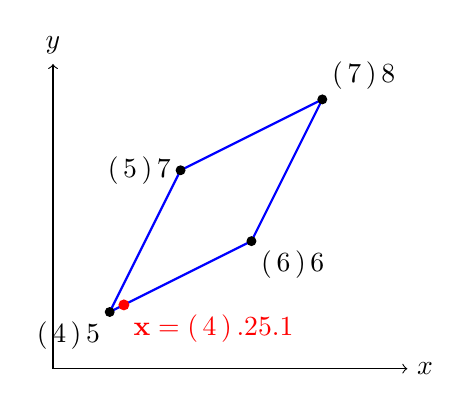
\begin{tikzpicture}[scale=0.9]
	\draw[->] (3.2,4.2) -- (8.2,4.2) node[right] {$x$};
	\draw[->] (3.2,4.2) -- (3.2,8.5) node[above] {$y$};
	
	\draw[thick, blue]
	(4,5) -- (5,7) -- (7,8) -- (6,6) -- cycle;
	
	\fill (4,5) circle (2pt) node[below left] {$\begin{pmatrix}4\\5\end{pmatrix}$};
	\fill (5,7) circle (2pt) node[left] {$\begin{pmatrix}5\\7\end{pmatrix}$};
	\fill (6,6) circle (2pt) node[below right] {$\begin{pmatrix}6\\6\end{pmatrix}$};
	\fill (7,8) circle (2pt) node[above right] {$\begin{pmatrix}7\\8\end{pmatrix}$};
	
	\fill[red] (4.2,5.1) circle (2.2pt)
	node[below right] {$\mathbf x=\begin{pmatrix}4.2\\5.1\end{pmatrix}$};
	
%	\node at (6.9,5.2) {$\begin{pmatrix}4\\5\end{pmatrix}+\mathcal P(B)$};
\end{tikzpicture}
\end{center}
				
	\end{proof}
\end{enumerate}

\newpage
\begin{enumerate}
	\item[\textbf{29-33}] 
%	Let
%	\[
%	B=
%	\begin{pmatrix}
%		2&0&1\\
%		1&1&0\\
%		0&1&2
%	\end{pmatrix},
%	\qquad
%	\Lambda=\mathcal L(B).
%	\]
%	For \(\mathbf x\in\mathbb R^3\), define its remainder modulo \(\Lambda\) by
%	\[
%	r_B(\mathbf x)=B\bigl(\{B^{-1}\mathbf x\}\bigr),
%	\]
%	where fractional parts are taken coordinatewise.
	We are given
\[
B=
\begin{pmatrix}
	2&0&1\\
	1&1&0\\
	0&1&2
\end{pmatrix},
\qquad
\Lambda=\mathcal L(B),
\qquad
r_B(\mathbf x)=B\bigl(\{B^{-1}\mathbf x\}\bigr).
\]
Compute \(B^{-1}\): Since $
\det(B)=5$, the matrix \(B\) is invertible, and
\[
B^{-1}
=
\frac15
\begin{pmatrix}
	2&1&-1\\
	-2&4&1\\
	1&-2&2
\end{pmatrix}
=
\begin{pmatrix}
	\frac25&\frac15&-\frac15\\[4pt]
	-\frac25&\frac45&\frac15\\[4pt]
	\frac15&-\frac25&\frac25
\end{pmatrix}.
\]

Recall that for a real number \(t\),
\[
\{t\}=t-\lfloor t\rfloor \in [0,1),
\]
and fractional parts are taken coordinatewise.
\end{enumerate}

\begin{center}
\begin{tikzpicture}[>=stealth, scale=0.85, transform shape]
	% Define common point styles
	\tikzstyle{pt} = [circle, fill=black, inner sep=1.8pt];
	\tikzstyle{targetpt} = [circle, fill=red, inner sep=1.8pt];
	
	% Macro to draw a 3D unit domain topologically (back faces first, then front)
	% #1: Line color, #2: Fill color
	\newcommand{\drawdomain}[2]{
		% Back faces (drawn first)
		\fill[#2, opacity=0.4] (0,0,0) -- (1,0,0) -- (1,1,0) -- (0,1,0) -- cycle; % Bottom
		\fill[#2, opacity=0.4] (0,0,0) -- (1,0,0) -- (1,0,1) -- (0,0,1) -- cycle; % Back-Left
		\fill[#2, opacity=0.4] (0,0,0) -- (0,1,0) -- (0,1,1) -- (0,0,1) -- cycle; % Back-Right
		
		% Included solid boundaries (intersecting the origin)
		\draw[#1, thick] (0,0,0) -- (1,0,0);
		\draw[#1, thick] (0,0,0) -- (0,1,0);
		\draw[#1, thick] (0,0,0) -- (0,0,1);
		
		% Front faces
		\fill[#2, opacity=0.4] (1,0,0) -- (1,1,0) -- (1,1,1) -- (1,0,1) -- cycle; % Front-Right
		\fill[#2, opacity=0.4] (0,1,0) -- (1,1,0) -- (1,1,1) -- (0,1,1) -- cycle; % Front-Left
		\fill[#2, opacity=0.4] (0,0,1) -- (1,0,1) -- (1,1,1) -- (0,1,1) -- cycle; % Top
		
		% Dashed Excluded Boundaries (x=1, y=1, z=1)
		\draw[#1, thick, dashed] (1,0,0) -- (1,1,0) -- (0,1,0);
		\draw[#1, thick, dashed] (1,0,0) -- (1,0,1) -- (0,0,1);
		\draw[#1, thick, dashed] (0,1,0) -- (0,1,1) -- (0,0,1);
		\draw[#1, thick, dashed] (1,1,0) -- (1,1,1);
		\draw[#1, thick, dashed] (1,0,1) -- (1,1,1);
		\draw[#1, thick, dashed] (0,1,1) -- (1,1,1);
	}
	
	% =========================================================================
	% LEFT SIDE: Standard Space R^3 (Variables: z, t, alpha)
	% =========================================================================
	\begin{scope}[xshift=0cm, yshift=0cm]
		% Define Standard Isometric Projection
		\begin{scope}[x={(-0.866cm, -0.5cm)}, y={(0.866cm, -0.5cm)}, z={(0cm, 1cm)}]
			% -- 3D Reference Grids --
			% Grid on the x1-x2 plane (Floor)
			\foreach \i in {1, 2, 3} {
				\draw[gray!30, very thin] (\i, 0, 0) -- (\i, 3.5, 0);
				\draw[gray!30, very thin] (0, \i, 0) -- (3.5, \i, 0);
			}
			
			% Grid on the x2-x3 plane (Left Wall)
			\foreach \i in {1, 2, 3} {
				\draw[gray!30, very thin] (0, \i, 0) -- (0, \i, 3.5);
				\draw[gray!30, very thin] (0, 0, \i) -- (0, 3.5, \i);
			}
			
			% Grid on the x1-x3 plane (Right Wall)
			\foreach \i in {1, 2, 3} {
				\draw[gray!30, very thin] (\i, 0, 0) -- (\i, 0, 3.5);
				\draw[gray!30, very thin] (0, 0, \i) -- (3.5, 0, \i);
			}
		
			% -- Axes --
			\draw[->, thick, gray] (0,0,0) -- (3.5,0,0) node[below] {$x_1$};
			\draw[->, thick, gray] (0,0,0) -- (0,3.5,0) node[below] {$x_2$};
			\draw[->, thick, gray] (0,0,0) -- (0,0,3.5) node[right] {$x_3$};
			
			% -- Highlighted Regions --
			% 1. Standard Fundamental Domain [0,1)^3 at origin
			\drawdomain{green!50!black}{green!15}
			\node[text=green!50!black] at (0.5, 0.5, -0.3) {\small $\mathcal{P}(I)$};
			
			% 2. Specific Translated Domain z + [0,1)^3 containing vector t
			% where z = (1, 1, 1)
			\begin{scope}[shift={(1,1,1)}]
				\drawdomain{blue}{blue!15}
			\end{scope}
			\node[text=blue] at (1.5, 1.5, 0.7) {\small $\mathbf{z} + [0,1)^3$};
			
			% -- Draw Integer Lattice Points Z^3 --
			\foreach \x in {0,...,2} {
				\foreach \y in {0,...,2} {
					\foreach \z in {0,...,2} {
						\fill[black] (\x,\y,\z) circle (1pt);
					}
				}
			}
			
			% -- Specific Vectors and Points --
			\coordinate (Z) at (1, 1, 1);
			\coordinate (T) at (1.6, 1.4, 1.8); % alpha = (0.6, 0.4, 0.8)
			\coordinate (Alpha) at (0.6, 0.4, 0.8);
			
			% Draw fractional vector alpha at origin
			\draw[->, ultra thick, red!80!black] (0,0,0) -- (Alpha) node[midway, right=2pt] {$\boldsymbol{\alpha}=\{B^{-1}\mathbf{x}\}$};
			
			% Draw vector t and offset
			\draw[->, thick, gray] (0,0,0) -- (T);
			\draw[->, thick, gray] (0,0,0) -- (Z);
			\draw[->, thick, red!80!black] (Z) -- (T);
			
			\filldraw[blue] (Z) circle (2pt) node[below left] {$\textbf{z}$}; 
			\filldraw[red] (T) circle (2pt) node[above] {$\textbf{t}$};
		\end{scope}
		
		\node[below, text width=8cm, align=center] at (0, -4.5) {\large $\mathcal L(I)$};
	\end{scope}
	
	% =========================================================================
	% MAPPING ARROW
	% =========================================================================
	\draw[->, line width=1.5pt] (3, 0) -- (7, 0) 
	node[midway, above, text=black] {\small $B = \begin{pmatrix} 2 & 0 & 1 \\ 1 & 1 & 0 \\ 0 & 1 & 2 \end{pmatrix}$};
	
	\draw[->, line width=1.5pt] (7, -1) -- (3, -1) 
	node[midway, below, text=black] {\small $B^{-1} = \frac{1}{5}\begin{pmatrix} 2 & 1 & -1 \\ -2 & 4 & 1 \\ 1 & -2 & 2 \end{pmatrix}$};
	
	% =========================================================================
	% RIGHT SIDE: Transformed Space R^3 (Variables: Bz, x, r_B(x))
	% =========================================================================
	\begin{scope}[xshift=10cm, yshift=0cm]
		% -- Background Standard Axes for Reference --
		\begin{scope}[x={(-0.866cm, -0.5cm)}, y={(0.866cm, -0.5cm)}, z={(0cm, 1cm)}]
			
			% -- 3D Background Reference Grids --
			
			% Floor (x1-x2 plane)
			\foreach \i in {1,...,4} {
				\draw[gray!20, very thin] (\i, 0, 0) -- (\i, 4.5, 0);
				\draw[gray!20, very thin] (0, \i, 0) -- (4.5, \i, 0);
			}
			
			% Left Wall (x2-x3 plane)
			\foreach \i in {1,...,4} {
				\draw[gray!20, very thin] (0, \i, 0) -- (0, \i, 4.5);
				\draw[gray!20, very thin] (0, 0, \i) -- (0, 4.5, \i);
			}
			
			% Right Wall (x1-x3 plane)
			\foreach \i in {1,...,4} {
				\draw[gray!20, very thin] (\i, 0, 0) -- (\i, 0, 4.5);
				\draw[gray!20, very thin] (0, 0, \i) -- (4.5, 0, \i);
			}
			
			\draw[->, thick, gray!40] (0,0,0) -- (5,0,0) node[below] {$x_1$};
			\draw[->, thick, gray!40] (0,0,0) -- (0,5,0) node[below] {$x_2$};
			\draw[->, thick, gray!40] (0,0,0) -- (0,0,5) node[right] {$x_3$};
		\end{scope}
		
		% We use a local scope with basis vectors mapped by matrix B
		% Be1 = 2e1 + 1e2 + 0e3  --> x = (-0.866, -1.5)
		% Be2 = 0e1 + 1e2 + 1e3  --> y = (0.866, 0.5)
		% Be3 = 1e1 + 0e2 + 2e3  --> z = (-0.866, 1.5)
		\begin{scope}[x={(-0.866cm, -1.5cm)}, y={(0.866cm, 0.5cm)}, z={(-0.866cm, 1.5cm)}]
			% -- 3D Background Reference Grids --
			
%			% Floor (x1-x2 plane)
%			\foreach \i in {1,...,3} {
%				\draw[red!50, very thin] (\i, 0, 0) -- (\i, 3.5, 0);
%				\draw[red!50, very thin] (0, \i, 0) -- (3.5, \i, 0);
%			}
%			
%			% Left Wall (x2-x3 plane)
%			\foreach \i in {1,...,3} {
%				\draw[red!50, very thin] (0, \i, 0) -- (0, \i, 3.5);
%				\draw[red!50, very thin] (0, 0, \i) -- (0, 3.5, \i);
%			}
%			
%			% Right Wall (x1-x3 plane)
%			\foreach \i in {1,...,3} {
%				\draw[red!50, very thin] (\i, 0, 0) -- (\i, 0, 3.5);
%				\draw[red!50, very thin] (0, 0, \i) -- (3.5, 0, \i);
%			}
		
			% -- Highlighted Regions --
			% 1. Fundamental Parallelepiped P(B) at origin
			\drawdomain{green!50!black}{green!15}
			\node[text=green!50!black] at (0.5, 0.5, -0.3) {\small $\mathcal{P}(B)$};
			
			% 2. Specific Translated Parallelepiped containing target vector x
			\begin{scope}[shift={(1,1,1)}]
				\drawdomain{blue}{blue!15}
			\end{scope}
			\node[text=blue] at (1.5, 1.5, 0.7) {\small $B\mathbf{z} + \mathcal{P}(B)$};
			
			% -- Draw Transformed Lattice Points Lambda --
			\foreach \i in {0,...,2} {
				\foreach \j in {0,...,2} {
					\foreach \k in {0,...,2} {
						\fill[black] (\i,\j,\k) circle (1pt);
					}
				}
			}
			
			% Define Coordinates in skewed basis
			\coordinate (BZ) at (1, 1, 1);
			\coordinate (X) at (1.6, 1.4, 1.8); 
			\coordinate (RB) at (0.6, 0.4, 0.8); 
			
			% -- Vectors and Points --
			% Draw the Remainder vector mapped inside P(B)
			\draw[->, ultra thick, red!80!black] (0,0,0) -- (RB) node[midway, below right] {$r_B(\mathbf{x})$};
			
			% Draw vectors to X
			\draw[->, thick, gray] (0,0,0) -- (X);
			\draw[->, thick, gray] (0,0,0) -- (BZ);
			\draw[->, thick, red!80!black] (BZ) -- (X);
			
			\filldraw[blue] (BZ) circle (2pt) node[below left] {$B\textbf{z}$}; 
			\filldraw[red] (X) circle (2pt) node[above] {$\textbf{x}$}; 
		\end{scope}
		
		% Label space
		\node[below, text width=8cm, align=center] at (0, -4.5) {\large $\Lambda = \mathcal L(B)$};
	\end{scope}
\end{tikzpicture}
\end{center}

\begin{enumerate}
	\setcounter{enumi}{28}
	\item\begin{proof}[\normalfont\color{magenta}\bfseries Sol]
		\begin{itemize}
			\item[($\mathbf x_1$)] Note that \[
			B^{-1}\mathbf x_1
			=
			\begin{pmatrix}
				\frac25&\frac15&-\frac15\\
				-\frac25&\frac45&\frac15\\
				\frac15&-\frac25&\frac25
			\end{pmatrix}
			\begin{pmatrix}
				\frac{26}{5}\\[2pt]
				\frac{37}{10}\\[2pt]
				-\frac75
			\end{pmatrix}
			=
			\begin{pmatrix}
				\frac{31}{10}\\[2pt]
				\frac35\\[2pt]
				-1
			\end{pmatrix}\implies
			\bigl\{B^{-1}\mathbf x_1\bigr\}
			=
			\begin{pmatrix}
				\left\{\frac{31}{10}\right\}\\[2pt]
				\left\{\frac35\right\}\\[2pt]
				\{-1\}
			\end{pmatrix}
			=
			\begin{pmatrix}
				\frac1{10}\\[2pt]
				\frac35\\[2pt]
				0
			\end{pmatrix}.
			\]
			Therefore
			\[
			r_B(\mathbf x_1)
			=
			B
			\begin{pmatrix}
				\frac1{10}\\[2pt]
				\frac35\\[2pt]
				0
			\end{pmatrix}
			=
			\begin{pmatrix}
				2&0&1\\
				1&1&0\\
				0&1&2
			\end{pmatrix}
			\begin{pmatrix}
				\frac1{10}\\[2pt]
				\frac35\\[2pt]
				0
			\end{pmatrix}
			=
			\begin{pmatrix}
				\frac15\\[2pt]
				\frac7{10}\\[2pt]
				\frac35
			\end{pmatrix}.
			\]
			\newpage
			\item[($\mathbf x_2$)] Note that
			\[
			B^{-1}\mathbf x_2
			=
			\begin{pmatrix}
				\frac25&\frac15&-\frac15\\
				-\frac25&\frac45&\frac15\\
				\frac15&-\frac25&\frac25
			\end{pmatrix}
			\begin{pmatrix}
				-\frac35\\[2pt]
				\frac{41}{10}\\[2pt]
				\frac{23}{10}
			\end{pmatrix}
			=
			\begin{pmatrix}
				\frac3{25}\\[2pt]
				\frac{199}{50}\\[2pt]
				-\frac{21}{25}
			\end{pmatrix}\implies
			\bigl\{B^{-1}\mathbf x_2\bigr\}
			=
			\begin{pmatrix}
				\frac3{25}\\[2pt]
				\frac{49}{50}\\[2pt]
				\frac4{25}
			\end{pmatrix}.
			\]
			Therefore
			\[
			r_B(\mathbf x_2)
			=
			B
			\begin{pmatrix}
				\frac3{25}\\[2pt]
				\frac{49}{50}\\[2pt]
				\frac4{25}
			\end{pmatrix}
			=
			\begin{pmatrix}
				\frac25\\[2pt]
				\frac{11}{10}\\[2pt]
				\frac{13}{10}
			\end{pmatrix}.
			\]
			\item[($\mathbf x_3$)] Note that
			\[
			B^{-1}\mathbf x_3
			=
			\begin{pmatrix}
				\frac25&\frac15&-\frac15\\
				-\frac25&\frac45&\frac15\\
				\frac15&-\frac25&\frac25
			\end{pmatrix}
			\begin{pmatrix}
				\frac{36}{5}\\[2pt]
				\frac{57}{10}\\[2pt]
				\frac35
			\end{pmatrix}
			=
			\begin{pmatrix}
				\frac{39}{10}\\[2pt]
				\frac95\\[2pt]
				-\frac35
			\end{pmatrix}\implies
			\bigl\{B^{-1}\mathbf x_3\bigr\}
			=
			\begin{pmatrix}
				\frac9{10}\\[2pt]
				\frac45\\[2pt]
				\frac25
			\end{pmatrix}.
			\]
			Therefore
			\[
			r_B(\mathbf x_3)
			=
			B
			\begin{pmatrix}
				\frac9{10}\\[2pt]
				\frac45\\[2pt]
				\frac25
			\end{pmatrix}
			=
			\begin{pmatrix}
				\frac{11}{5}\\[2pt]
				\frac{17}{10}\\[2pt]
				\frac85
			\end{pmatrix}.
			\]
		\end{itemize}
		So the remainders are
		\[
		\boxed{
			r_B(\mathbf x_1)=
			\begin{pmatrix}
				\frac15\\[2pt]
				\frac7{10}\\[2pt]
				\frac35
			\end{pmatrix},
			\qquad
			r_B(\mathbf x_2)=
			\begin{pmatrix}
				\frac25\\[2pt]
				\frac{11}{10}\\[2pt]
				\frac{13}{10}
			\end{pmatrix},
			\qquad
			r_B(\mathbf x_3)=
			\begin{pmatrix}
				\frac{11}{5}\\[2pt]
				\frac{17}{10}\\[2pt]
				\frac85
			\end{pmatrix}.
		}
		\]
	\end{proof}
	\item \begin{proof}[\normalfont\color{magenta}\bfseries Sol]
	\begin{itemize}
		\item[($\mathbf x_1$)] \[
		\mathbf y_1
		=
		\mathbf x_1-r_B(\mathbf x_1)
		=
		\begin{pmatrix}
			\frac{26}{5}\\[2pt]
			\frac{37}{10}\\[2pt]
			-\frac75
		\end{pmatrix}
		-
		\begin{pmatrix}
			\frac15\\[2pt]
			\frac7{10}\\[2pt]
			\frac35
		\end{pmatrix}
		=
		\begin{pmatrix}
			5\\[2pt]
			3\\[2pt]
			-2
		\end{pmatrix}.
		\]
		Also,
		\[
		\mathbf y_1
		=
		B
		\begin{pmatrix}
			3\\0\\-1
		\end{pmatrix},
		\]
		so \(\mathbf y_1\in\Lambda\).
		\item[($\mathbf x_2$)] \[
		\mathbf y_2
		=
		\mathbf x_2-r_B(\mathbf x_2)
		=
		\begin{pmatrix}
			-\frac35\\[2pt]
			\frac{41}{10}\\[2pt]
			\frac{23}{10}
		\end{pmatrix}
		-
		\begin{pmatrix}
			\frac25\\[2pt]
			\frac{11}{10}\\[2pt]
			\frac{13}{10}
		\end{pmatrix}
		=
		\begin{pmatrix}
			-1\\[2pt]
			3\\[2pt]
			1
		\end{pmatrix}.
		\]
		Also,
		\[
		\mathbf y_2
		=
		B
		\begin{pmatrix}
			0\\3\\-1
		\end{pmatrix},
		\]
		so \(\mathbf y_2\in\Lambda\).
		\item[($\mathbf x_3$)] \[
		\mathbf y_3
		=
		\mathbf x_3-r_B(\mathbf x_3)
		=
		\begin{pmatrix}
			\frac{36}{5}\\[2pt]
			\frac{57}{10}\\[2pt]
			\frac35
		\end{pmatrix}
		-
		\begin{pmatrix}
			\frac{11}{5}\\[2pt]
			\frac{17}{10}\\[2pt]
			\frac85
		\end{pmatrix}
		=
		\begin{pmatrix}
			5\\[2pt]
			4\\[2pt]
			-1
		\end{pmatrix}.
		\]
		Also,
		\[
		\mathbf y_3
		=
		B
		\begin{pmatrix}
			3\\1\\-1
		\end{pmatrix},
		\]
		so \(\mathbf y_3\in\Lambda\).
	\end{itemize}
	Thus
	\[
	\boxed{
		\mathbf y_1=
		\begin{pmatrix}
			5\\3\\-2
		\end{pmatrix},
		\qquad
		\mathbf y_2=
		\begin{pmatrix}
			-1\\3\\1
		\end{pmatrix},
		\qquad
		\mathbf y_3=
		\begin{pmatrix}
			5\\4\\-1
		\end{pmatrix}.
	}
	\]
	\end{proof}
\item \begin{proof}[\normalfont\color{magenta}\bfseries Sol]
Two vectors lie in the same coset modulo \(\Lambda\) if and only if they have the same remainder modulo \(\Lambda\).
From part (29),
\[
r_B(\mathbf x_1)\neq r_B(\mathbf x_2),\qquad
r_B(\mathbf x_1)\neq r_B(\mathbf x_3),\qquad
r_B(\mathbf x_2)\neq r_B(\mathbf x_3).
\]
Therefore no two of the vectors lie in the same coset modulo \(\Lambda\).
Hence
\[
\boxed{\text{none of the pairs }(\mathbf x_1,\mathbf x_2),\ (\mathbf x_1,\mathbf x_3),\ (\mathbf x_2,\mathbf x_3)\text{ lie in the same coset mod }\Lambda.}
\]
\end{proof}
\item \begin{proof}[\normalfont\color{magenta}\bfseries Sol]
Since no pair lies in the same coset modulo \(\Lambda\), there are no such pairs. Hence there is no pair \((i,j)\) with
\[
\mathbf x_i-\mathbf x_j\in\Lambda.
\]

Equivalently, one may check directly that none of the pairwise differences has integer \(B\)-coordinates:
\[
B^{-1}(\mathbf x_1-\mathbf x_2)
=
\begin{pmatrix}
	\frac{149}{50}\\[2pt]
	-\frac{169}{50}\\[2pt]
	-\frac4{25}
\end{pmatrix},
\quad
B^{-1}(\mathbf x_1-\mathbf x_3)
=
\begin{pmatrix}
	-\frac45\\[2pt]
	-\frac65\\[2pt]
	-\frac25
\end{pmatrix},
\quad
B^{-1}(\mathbf x_2-\mathbf x_3)
=
\begin{pmatrix}
	-\frac{189}{50}\\[2pt]
	\frac{109}{50}\\[2pt]
	-\frac6{25}
\end{pmatrix},
\]
and none of these vectors lies in \(\mathbb Z^3\). Therefore none of the differences belongs to \(\Lambda\).
\end{proof}
\item \begin{proof}[\normalfont\color{magenta}\bfseries Sol]
For each \(\mathbf x_i\), we computed
\[
\mathbf x_i=\mathbf y_i+r_B(\mathbf x_i),
\qquad
\mathbf y_i\in\Lambda.
\]
Moreover, since
\[
\{B^{-1}\mathbf x_i\}\in[0,1)^3,
\]
each remainder
\[
r_B(\mathbf x_i)=B\bigl(\{B^{-1}\mathbf x_i\}\bigr)
\]
lies in the fundamental parallelepiped
\[
\mathcal P(B)=\{B\boldsymbol\alpha:\boldsymbol\alpha\in[0,1)^3\}.
\]
Thus each \(\mathbf x_i\) has been written in the form
\[
\mathbf x_i=\mathbf y_i+\mathbf p_i,
\qquad
\mathbf y_i\in\Lambda,\ \mathbf p_i\in\mathcal P(B).
\]

The fact that the three remainders are different shows that the three vectors lie in different cosets modulo \(\Lambda\). In other words, the remainder \(\mathbf p\in\mathcal P(B)\) serves as the unique representative of the coset \(\mathbf x+\Lambda\).

So these calculations concretely illustrate the theorem:

\begin{quote}
	Every \(\mathbf x\in\mathbb R^3\) can be written uniquely as
	\[
	\mathbf x=\mathbf y+\mathbf p,
	\qquad
	\mathbf y\in\Lambda,\ \mathbf p\in\mathcal P(B).
	\]
\end{quote}

Here the lattice part is \(\mathbf y_i\), and the unique fundamental-domain representative is \(r_B(\mathbf x_i)\).
\end{proof}
\end{enumerate}
